%\subsection{Experimental Uncertainties}
\label{subsec:exp_uncer}


\subsection{Baseline uncertainties}
\label{subsubsec:baseline_unc}
The summary of experimental uncertainties is presented in Tab.~\ref{tab:syst_summary_sources_1} to \ref{tab:syst_summary_sources_3}.
 
\begin{table}[!hp]
  \caption{ Qualitative summary of the systematic uncertainties included in this analysis. }
  \label{tab:syst_summary_sources_1}
  \centering
  \footnotesize
  \begin{center}
    \begin{tabular}{|l|l|l|l|}
      \hline
      Source        & Description                     & Analysis Name                         & Notes              \\ \hline
      Electrons     & Energy scale                    &  EG\_SCALE\_ALL                     & \\ 
      Electrons     & Energy resolution               &  EG\_RESOLUTION\_ALL                & \\ 
      Electrons     & Trigger                        &  EL\_EFF\_Trigger\_TOTAL\_1NPCOR\_PLUS\_UNCOR                    & \\ 
      Electrons     & ID efficiency SF                &  EL\_EFF\_ID\_TOTAL\_1NPCOR\_PLUS\_UNCOR  & \\
      Electrons     & Isolation efficiency SF                &   EL\_EFF\_Iso\_TOTAL\_1NPCOR\_PLUS\_UNCOR  & \\
      Electrons     & Reconstruction efficiency SF                &   EL\_EFF\_Reco\_TOTAL\_1NPCOR\_PLUS\_UNCOR  & \\ \hline
      Muons         & \pt\ scale                       &   MUONS\_SCALE                       & \\ 
      Muons         & \pt\ scale (charge dependent)          &   MUON\_SAGITTA\_RHO                    & \\ 
      Muons         & \pt\ scale (charge dependent)          &   MUON\_SAGITTA\_RESBIAS                     & \\ 
      Muons         & \pt\ resolution MS               &   MUONS\_MS                          & \\ 
      Muons         & \pt\ resolution ID               &   MUONS\_ID                          & \\ 
      Muons         & Isolation efficiency SF         &   MUON\_ISO\_SYS                     & \\ 
      Muons         & Isolation efficiency SF         &   MUON\_ISO\_STAT                    & \\ 
      Muons         & Muon reco \& ID efficiency SF               &   MUONS\_EFF\_STAT                          & \\ 
      Muons         & Muon reco \& ID efficiency SF               &   MUONS\_EFF\_STAT\_LOWPT                          & \\ 
      Muons         & Muon reco \& ID efficiency SF               &   MUONS\_EFF\_SYST                          & \\ 
      Muons         & Muon reco \& ID efficiency SF               &   MUONS\_EFF\_SYST\_LOWPT                          & \\ 
      Muons         & Track-to-vertex association efficiency SF         &   MUON\_TTVA\_SYS                     & \\ 
      Muons         & Track-to-vertex association efficiency SF         &   MUON\_TTVA\_STAT                     & \\ 
      Muons         & Trigger         &   MUON\_EFF\_TrigSystUncertainty   & \\
      Muons         & Trigger         &   MUON\_EFF\_TrigStatUncertainty   & \\    \hline
        %MET           & Trigger scale factor            &   METTrigStat                        & \\
        %MET           & Trigger scale factor            &   METTrigTop                         & \\
      MET           & Soft term                       &   MET\_SoftTrk\_ResoPerp             & \\ 
      MET           & Soft term                       &   MET\_SoftTrk\_ResoPara             & \\ 
      MET           & Soft term                       &   MET\_SoftTrk\_Scale              & \\
      %MET           & Jet track uncertainties         &   MET\_JetTrk\_Scale                 & \\ 
      \hline
      \end{tabular}
    \end{center}
  \end{table}


\begin{table}[!hp]
  \caption{ Qualitative summary of the systematic uncertainties included in this analysis. }
  \label{tab:syst_summary_sources_2}
  \centering
  \footnotesize
  \begin{center}
    \begin{tabular}{|l|l|l|l|}
      \hline
      Source        & Description                     & Analysis Name                         & Notes              \\ \hline
      Small-R Jets  & JES category reduction            &  JET\_CR\_JET\_BJES\_Response                             & \\ 
      Small-R Jets  & JES category reduction            &  JET\_CR\_JET\_EffectiveNP\_Detector1                     & \\ 
      Small-R Jets  & JES category reduction            &  JET\_CR\_JET\_EffectiveNP\_Detector2                     & \\ 
      Small-R Jets  & JES category reduction            &  JET\_CR\_JET\_EffectiveNP\_Mixed1                        & \\ 
      Small-R Jets  & JES category reduction            &  JET\_CR\_JET\_EffectiveNP\_Mixed2                        & \\ 
      Small-R Jets  & JES category reduction            &  JET\_CR\_JET\_EffectiveNP\_Mixed3                        & \\ 
      Small-R Jets  & JES category reduction            &  JET\_CR\_JET\_EffectiveNP\_Modelling1                    & \\ 
      Small-R Jets  & JES category reduction            &  JET\_CR\_JET\_EffectiveNP\_Modelling2                    & \\ 
      Small-R Jets  & JES category reduction            &  JET\_CR\_JET\_EffectiveNP\_Modelling3                    & \\ 
      Small-R Jets  & JES category reduction            &  JET\_CR\_JET\_EffectiveNP\_Modelling4                    & \\ 
      Small-R Jets  & JES category reduction            &  JET\_CR\_JET\_EffectiveNP\_Statistical1                  & \\ 
      Small-R Jets  & JES category reduction            &  JET\_CR\_JET\_EffectiveNP\_Statistical2                  & \\ 
      Small-R Jets  & JES category reduction            &  JET\_CR\_JET\_EffectiveNP\_Statistical3                  & \\ 
      Small-R Jets  & JES category reduction            &  JET\_CR\_JET\_EffectiveNP\_Statistical4                  & \\ 
      Small-R Jets  & JES category reduction            &  JET\_CR\_JET\_EffectiveNP\_Statistical5                  & \\ 
      Small-R Jets  & JES category reduction            &  JET\_CR\_JET\_EffectiveNP\_Statistical6                  & \\ 
      Small-R Jets  & JES category reduction            &  JET\_CR\_JET\_Flavor\_Composition                        & \\ 
      Small-R Jets  & JES category reduction            &  JET\_CR\_JET\_Flavor\_Response                           & \\ 
      Small-R Jets  & JES category reduction            &  JET\_CR\_JET\_Pileup\_OffsetMu                           & \\ 
      Small-R Jets  & JES category reduction            &  JET\_CR\_JET\_Pileup\_OffsetNPV                          & \\ 
      Small-R Jets  & JES category reduction            &  JET\_CR\_JET\_Pileup\_PtTerm                             & \\ 
      Small-R Jets  & JES category reduction            &  JET\_CR\_JET\_Pileup\_RhoTopology                        & \\ 
      Small-R Jets  & JES category reduction            &  JET\_CR\_JET\_PunchThrough\_MC16                         & \\ 
      Small-R Jets  & JES category reduction            &  JET\_CR\_JET\_SingleParticle\_HighPt                     & \\ 
      Small-R Jets  & JES category reduction            &  JET\_CR\_JET\_EtaIntercalibration\_TotalStat             & \\ 
      Small-R Jets  & JES category reduction            &  JET\_CR\_JET\_EtaIntercalibration\_Modelling             & \\ 
      Small-R Jets  & JES category reduction            &  JET\_CR\_JET\_EtaIntercalibration\_NonClosure\_highE     & \\ 
      Small-R Jets  & JES category reduction            &  JET\_CR\_JET\_EtaIntercalibration\_NonClosure\_negEta    & \\ 
      Small-R Jets  & JES category reduction            &  JET\_CR\_JET\_EtaIntercalibration\_NonClosure\_posEta    & \\ 
        \hline
        Small-R Jets  & JER                  &  JET\_CR\_JET\_JER\_DataVsMC                  & \\ 
        Small-R Jets  & JER                  &  JET\_CR\_JET\_JER\_EffectiveNP\_1            & \\ 
        Small-R Jets  & JER                  &  JET\_CR\_JET\_JER\_EffectiveNP\_2            & \\ 
        Small-R Jets  & JER                  &  JET\_CR\_JET\_JER\_EffectiveNP\_3            & \\ 
        Small-R Jets  & JER                  &  JET\_CR\_JET\_JER\_EffectiveNP\_4            & \\ 
        Small-R Jets  & JER                  &  JET\_CR\_JET\_JER\_EffectiveNP\_5            & \\ 
        Small-R Jets  & JER                  &  JET\_CR\_JET\_JER\_EffectiveNP\_6            & \\ 
        Small-R Jets  & JER                  &  JET\_CR\_JET\_JER\_EffectiveNP\_7restTerm    & \\ 
        \hline
        Small-R Jets  & JVT                  &  JET\_JvtEfficiency    & \\
%        Small-R Jets  & fJVT                  &  JET\_fJvtEfficiency    & \\ 
        \hline
        \end{tabular}
    \end{center}
  \end{table}


\begin{table}[!hp]
  \caption{ Qualitative summary of the systematic uncertainties included in this analysis. }
  \label{tab:syst_summary_sources_3}
  \centering
  \footnotesize
  \begin{center}
    \begin{tabular}{|l|l|l|l|}
      \hline
      Source        & Description                     & Analysis Name                         & Notes              \\ \hline
      Large-R Jets  & \pt scale                       & FATJET\_Medium\_JET\_Rtrk\_Baseline\_pT                            &  \\
      %Large-R Jets  & \pt scale                       & FATJET\_Medium\_JET\_Rtrk\_Closure\_pT                             &  \\
      Large-R Jets  & \pt scale                       & FATJET\_Medium\_JET\_Rtrk\_Modelling\_pT                           &  \\
      Large-R Jets  & \pt scale                       & FATJET\_Medium\_JET\_Rtrk\_TotalStat\_pT                           &  \\
      Large-R Jets  & \pt scale                       & FATJET\_Medium\_JET\_Rtrk\_Tracking\_pT                            &  \\

      Large-R Jets  & \pt scale                       & FATJET\_BJT\_JET\_EtaIntercalibration\_Modelling      & \\
      Large-R Jets  & \pt scale                       & FATJET\_BJT\_JET\_Flavor\_Composition                 & \\
      Large-R Jets  & \pt scale                       & FATJET\_BJT\_JET\_Flavor\_Response                    & \\

      Large-R Jets  & Mass resolution                 & FATJET\_JMR                            & \\\hline
      Large-R Jets  & JER                             & FATJET\_JER                            & \\\hline

%
      B-tagging     & Flavor tagging scale factors    &  FT\_EFF\_Eigen\_B\_0\_AntiKt4PFlowJets                                & \\
      B-tagging     & Flavor tagging scale factors    &  FT\_EFF\_Eigen\_B\_1\_AntiKt4PFlowJets                                & \\
      B-tagging     & Flavor tagging scale factors    &  FT\_EFF\_Eigen\_B\_2\_AntiKt4PFlowJets                                & \\
      B-tagging     & Flavor tagging scale factors    &  FT\_EFF\_Eigen\_C\_0\_AntiKt4PFlowJets                                & \\
      B-tagging     & Flavor tagging scale factors    &  FT\_EFF\_Eigen\_C\_1\_AntiKt4PFlowJets                                & \\
      B-tagging     & Flavor tagging scale factors    &  FT\_EFF\_Eigen\_C\_2\_AntiKt4PFlowJets                                & \\
      B-tagging     & Flavor tagging scale factors    &  FT\_EFF\_Eigen\_C\_3\_AntiKt4PFlowJets                                & \\
      B-tagging     & Flavor tagging scale factors    &  FT\_EFF\_Eigen\_Light\_0\_AntiKt4PFlowJets                            & \\
      B-tagging     & Flavor tagging scale factors    &  FT\_EFF\_Eigen\_Light\_1\_AntiKt4PFlowJets                            & \\
      B-tagging     & Flavor tagging scale factors    &  FT\_EFF\_Eigen\_Light\_2\_AntiKt4PFlowJets                            & \\
      B-tagging     & Flavor tagging scale factors    &  FT\_EFF\_Eigen\_Light\_3\_AntiKt4PFlowJets                            & \\
      B-tagging     & Flavor tagging scale factors    &  FT\_EFF\_extrapolation\_AntiKt4PFlowJets                              & \\
      B-tagging     & Flavor tagging scale factors    &  FT\_EFF\_extrapolation\_from\_charm\_AntiKt4PFlowJets                 & \\

      \hline                          
      Pileup reweighting & PRW\_DATASF & PRW\_DATASF &\\ 
      Luminosity & LumiNP & ATLAS\_LUMI\_2015\_2018 & \\
\hline
\end{tabular}
    \end{center}
  \end{table}

\clearpage
\subsubsection*{Luminosity}
%The luminosity uncertainty is applied to those backgrounds estimated from simulation and the signal samples.
Luminosity uncertainty is applied to both the signal and background MC samples.
The uncertainties on the integrated luminosity for the datasets are as follows:
\begin{itemize}
    \item 2015+2016 dataset: 2.1\%
    \item 2017 dataset: 2.4\%
    \item 2018 dataset: 2.0\%
    \item Combined Run-2 dataset (2015-2018): 1.7\%
\end{itemize}
Reference:~\cite{AtlasLumiRun2}.


\subsubsection*{Pileup reweighting}
The uncertainty associated with the pileup reweighting is accounted for as \texttt{PRW\_DATASF}~\cite{ExtendedPileupReweighting}. 
A variation in the pileup reweighting of MC simulations is included to address the uncertainty in the ratio of the predicted to the measured inelastic cross-section within the fiducial volume defined by $M_X > 13\,\GeV$, where $M_X$ is the mass of the non-diffractive hadronic system~\cite{STDM-2015-05}.


\subsubsection*{Trigger}
Systematic uncertainties on the efficiency of the electron or muon triggers are evaluated using the tag-and-probe method, applied to both the signal and background MC samples. Efficiencies are obtained using the \texttt{ElectronEfficiencyCorrection}~\cite{AsgElectronEfficiencyCorrectionTool} and \texttt{MuonEfficiencyCorrections}~\cite{TrigMuonEfficiency} tools. The uncertainty in the \met trigger is derived from the scale factor estimation, incorporating statistical contributions and efficiency discrepancies between MC samples, specifically \ttbar and \Wjets backgrounds~\cite{ATLAS-CONF-2016-091, Masubuchi:2151844}. Upon evaluation, trigger uncertainties were found to be less than 1\% and were subsequently excluded from the final fit results due to their minimal impact.

\subsubsection*{Muons and electrons}
The following systematic uncertainties are applied to electrons and muons for simulation-based estimations:

\begin{itemize}
    \item \textbf{Identification and reconstruction efficiencies:} Measured using the tag-and-probe method centered around the $Z$ mass peak.
    \item \textbf{Isolation efficiency:} The scale factor and its uncertainty are derived via the tag-and-probe method, also utilizing the $Z$ mass peak.
    \item \textbf{Energy and Momentum scales:} Determined through the $Z$ mass line shape analysis, with contributions from the CP groups.
    \item \textbf{Track-to-vertex association efficiency:} This applies solely to muons.
\end{itemize}

%%%Implementation of these uncertainties is carried out through the following tools:
%%%\begin{itemize}
%%%    \item \texttt{ElectronPhotonFourMomentumCorrection} \cite{EgammaCalibration}
%%%    \item \texttt{ElectronEfficiencyCorrection} \cite{AsgElectronEfficiencyCorrectionTool}
%%%    \item \texttt{MuonMomentumCorrections} and \texttt{MuonEfficiencyCorrections} \cite{MCPAnalysisGuidelines}
%%%\end{itemize}

\subsubsection*{Missing transverse energy}

The missing transverse energy (\met) is calculated using physics objects, as outlined in Section~\ref{sec:MET_reconstruction}. 
Systematic uncertainties in the reconstructed components, such as the jet energy scale, directly affect the \met and represent its primary sources of uncertainty. Additionally, the uncertainty known as the ``Soft Term,'' which arises from tracks in the inner detector not associated with any reconstructed objects, is also considered. The resolution and scale of the Soft Term are varied within their respective uncertainties to assess their impact on the overall \met uncertainty, utilizing the \texttt{METUtilities} tool~\cite{METUtilSystematics}.

\subsubsection*{Small-$R$ Jet Energy Scale and Resolution Uncertainty}
The jet energy scale (JES) and resolution (JER) for small-$R$ jets are determined by comparing the response in MC samples to data across various bins in kinematic phase space.
% employing the \texttt{JetUncertainties} tool~\cite{JetUncertainties}. 
The analysis utilizes the configuration \texttt{R4\_CategoryReduction\_SimpleJER}, which incorporates 30 JES and 8 JER uncertainty components. These uncertainties are particularly significant in the boosted analysis due to their impact on the calculation of \met. 
The efficiency uncertainty of the Jet Vertex Tagger (JVT) is evaluated; however, since its effect was found to be below 1\%, it was excluded from the final fit.

\subsubsection*{Large-$R$ Jet Energy Scale and Resolution Uncertainty}
\label{sec:fatjetUncert}
%More information are provided in the main twiki for the large-R jets recommendations \cite{JSSrecommendation2}.
The uncertainties for the large-$R$ jet energy scale are incorporated according to the prescription provided by the jet substructure group.
% as included in the \texttt{JetUncertainties} package~\cite{JSSrecommendation}. 
The uncertainty related to the jet \pt scale is assessed through the Rtrk method, which involves comparing the ratio of jet \pt to track-jet \pt in dijet data versus simulation. Beyond the ``baseline'' uncertainty, additional considerations include uncertainties related to track measurements (``Tracking''), variations between Pythia and Sherpa dijet simulations (``Modelling''), and the statistical uncertainty in dijet data (``TotalStat'').

%The large-$R$ jet resolution uncertainty recommendation is not included in the \texttt{JetUncertainties} package~\cite{JSSrecommendation}.
%As a \pt resolution uncertainty, jet \pt is smeared by Gaussian with 2\% width.

\subsubsection*{B-tagging systematics}
%Systematic uncertainties related to $b$-tagging are accounted for as described in~\cite{BTagCalib}. 
Systematic uncertainties related to $b$-tagging arise from scaling factors designed to correct discrepancies in $b$-tagging efficiency between data and MC simulations. Separate scale factors and their respective systematic uncertainties are determined for jets originating from $b$-quarks, $c$-quarks, and light-flavor quarks, based on various measurements.
 
%%%
\subsection{$W/Z$-tagging efficiency SF Uncertainty}
%%%%%%%%%%%%%%%%%
%  Boson Tagger 
%%%%%%%%%%%%%%%%%
%\subsubsection{Boson Tagger}
\label{subsec:bkg_uncer_vtagger}

For the uncertainties associated with the boson tagger's background efficiency, we consider both the large-\(R\) jet-related uncertainties and the modelling uncertainties from multi-jet and $\gamma$+jets. 
The modelling uncertainties are estimated by comparing the nominal Pythia 8 and Sherpa samples against alternative Sherpa and Pythia 8 samples for multi-jet and $\gamma$+jets, respectively.
For more on how the tagger is defined, see \cite{ATL-PHYS-PUB-2020-017}.

Systematic uncertainties associated with the scale factors, which assess the boson tagger's relative performance in data versus MC, are thoroughly evaluated. 
These uncertainties encompass various aspects. For background uncertainties, factors such as matrix element variations, hadronization, radiation effects, and the impact of dijets or $\gamma$+jets events are considered. Signal uncertainties include considerations like the extrapolation at high-\(\pT\).

Further details on these recommendations are available on the central CP twiki \cite{JSSrecommendationSF}. Plots illustrating the impact of uncertainties on the Data/MC ratio for the \olep channel are presented in Figure \ref{fig:1LepVTaggerUnc}.

%%%
%%%For the boson tagger uncertainties related to the background efficiency measurement, the large-R jet related uncertainties as well as multi-jet and $\gamma$+jets modelling uncertainties are considered. 
%%%The modelling uncertainties are estimated from the nominal Pythia 8 and Sherpa sample in comparison to the alternative  Sherpa and Pythia 8 samples for multijet and $\gamma$+jets respectively. 
%%%For more on how the tagger is defined, see \cite{ATL-PHYS-PUB-2020-017}.
%%%
%%%Systematic uncertainties related to the scale factors used to quantify the relative performance 
%%%of the boson tagger in data versus MC are also considered; 
%%%detailed information are provided in the main recommendation twiki from the CP group \cite{JSSrecommendationSF}.
%%%
%%%In Figure \ref{fig:2lep_bkgUnc_BT} Data/MC ratios are plotted as a function of the mass of the tagging jets 
%%%for the different merged analysis regions of the 2-lepton channel and for the different boson tagger related uncertainties. 
%%%They are related to both background uncertainties, like matrix element, hadronisation, radiation effects,
%%%impact of dijets or $\gamma$+jets events, both to signal uncertainties, like extrapolation at high-\pT or
%%%extrapolation to the Z boson. Further details can be found on the central CP twiki for the recommendations
%%%\cite{JSSrecommendationSF}.
%%%The largest systematic uncertainty is related to the $\gamma$+jets modelling and is seen in the HP signal region. 
%%%In the merged CR the major systematic source is related to the efficiency uncertainty of the 80\% tagger working point 
%%%while in the LP SR major systematic sources (still less than 5\%) are related to the $\gamma$+jets modelling 
%%%and the efficiency uncertainty of the 50\% tagger working point. 
%%%The fact that the efficiency uncertainty of the 50\% tagger working point is relevant in the LP SR is not surprising 
%%%given the SF calculation in this region, which is defined as: 
%%%
%%%    \begin{equation}
%%%        SF_{LP} = \frac{\epsilon_{loose}SF_{eff,loose}- \epsilon_{tight}SF_{eff,tight} }{ \epsilon_{loose}- \epsilon_{tight}}
%%%    \end{equation}        
%%%.
%%%
%%%Similar plots showing the impact of the effect of the uncertainties around the Data/MC ratio 
%%%for the \olep channel are shown in Figure \ref{fig:1LepVTaggerUnc};
%%%the impact of all the SF related uncertainties on the MC shapes of the signal and bkg samples
%%%in the \zlep channel are shown in Figure \ref{fig:0LepVTaggerUnc}.

\begin{figure}[ht]
    \centering
    \begin{subfigure}[b]{0.3\textwidth}
        \centering
        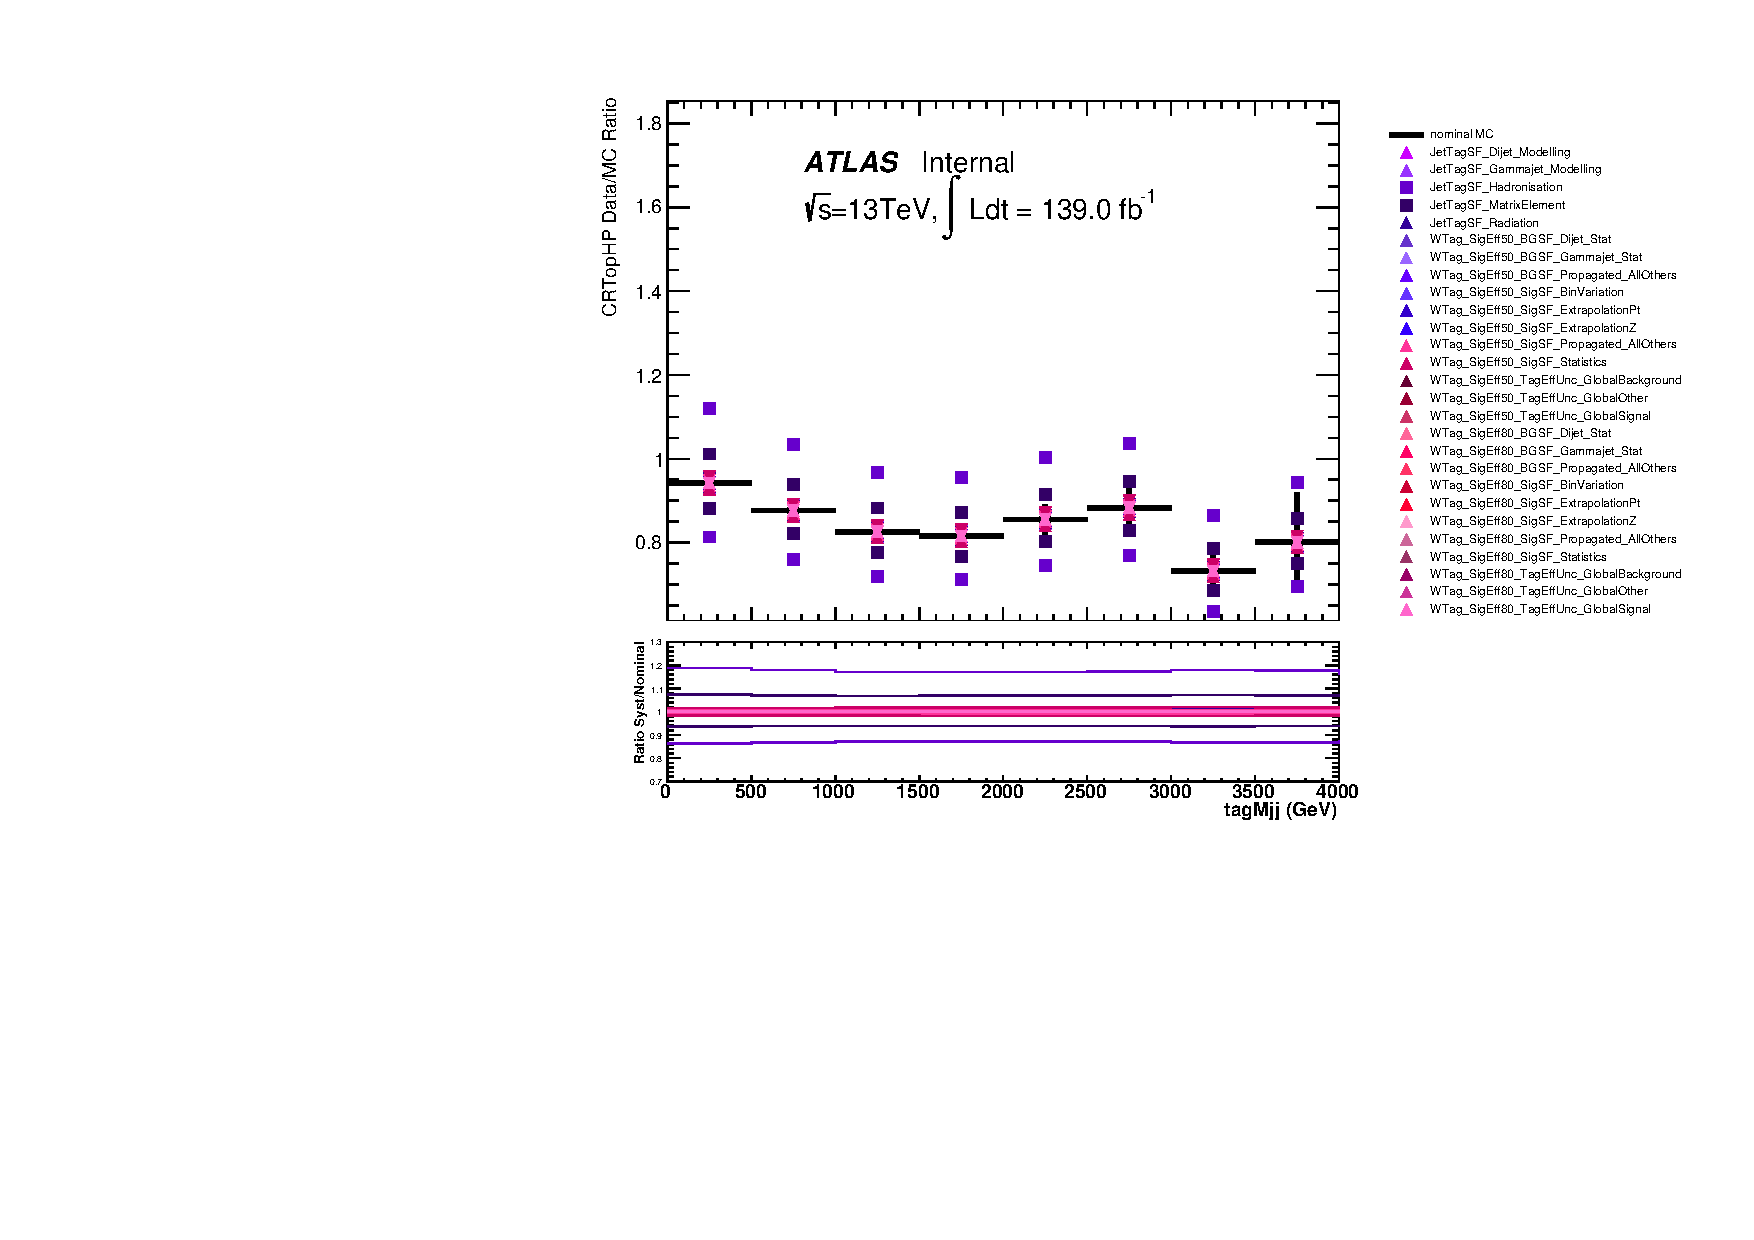
\includegraphics[width=\textwidth]{figures/1lep/VTaggerUnc/VTagCRTopHPtagMjj_SystBreakDown.pdf}
        \caption{Merged HP TopCR}
        \label{fig:MergedHPTopCR}
    \end{subfigure}
%    \hfill % This adds a bit of horizontal spacing between figures
    \begin{subfigure}[b]{0.3\textwidth}
        \centering
        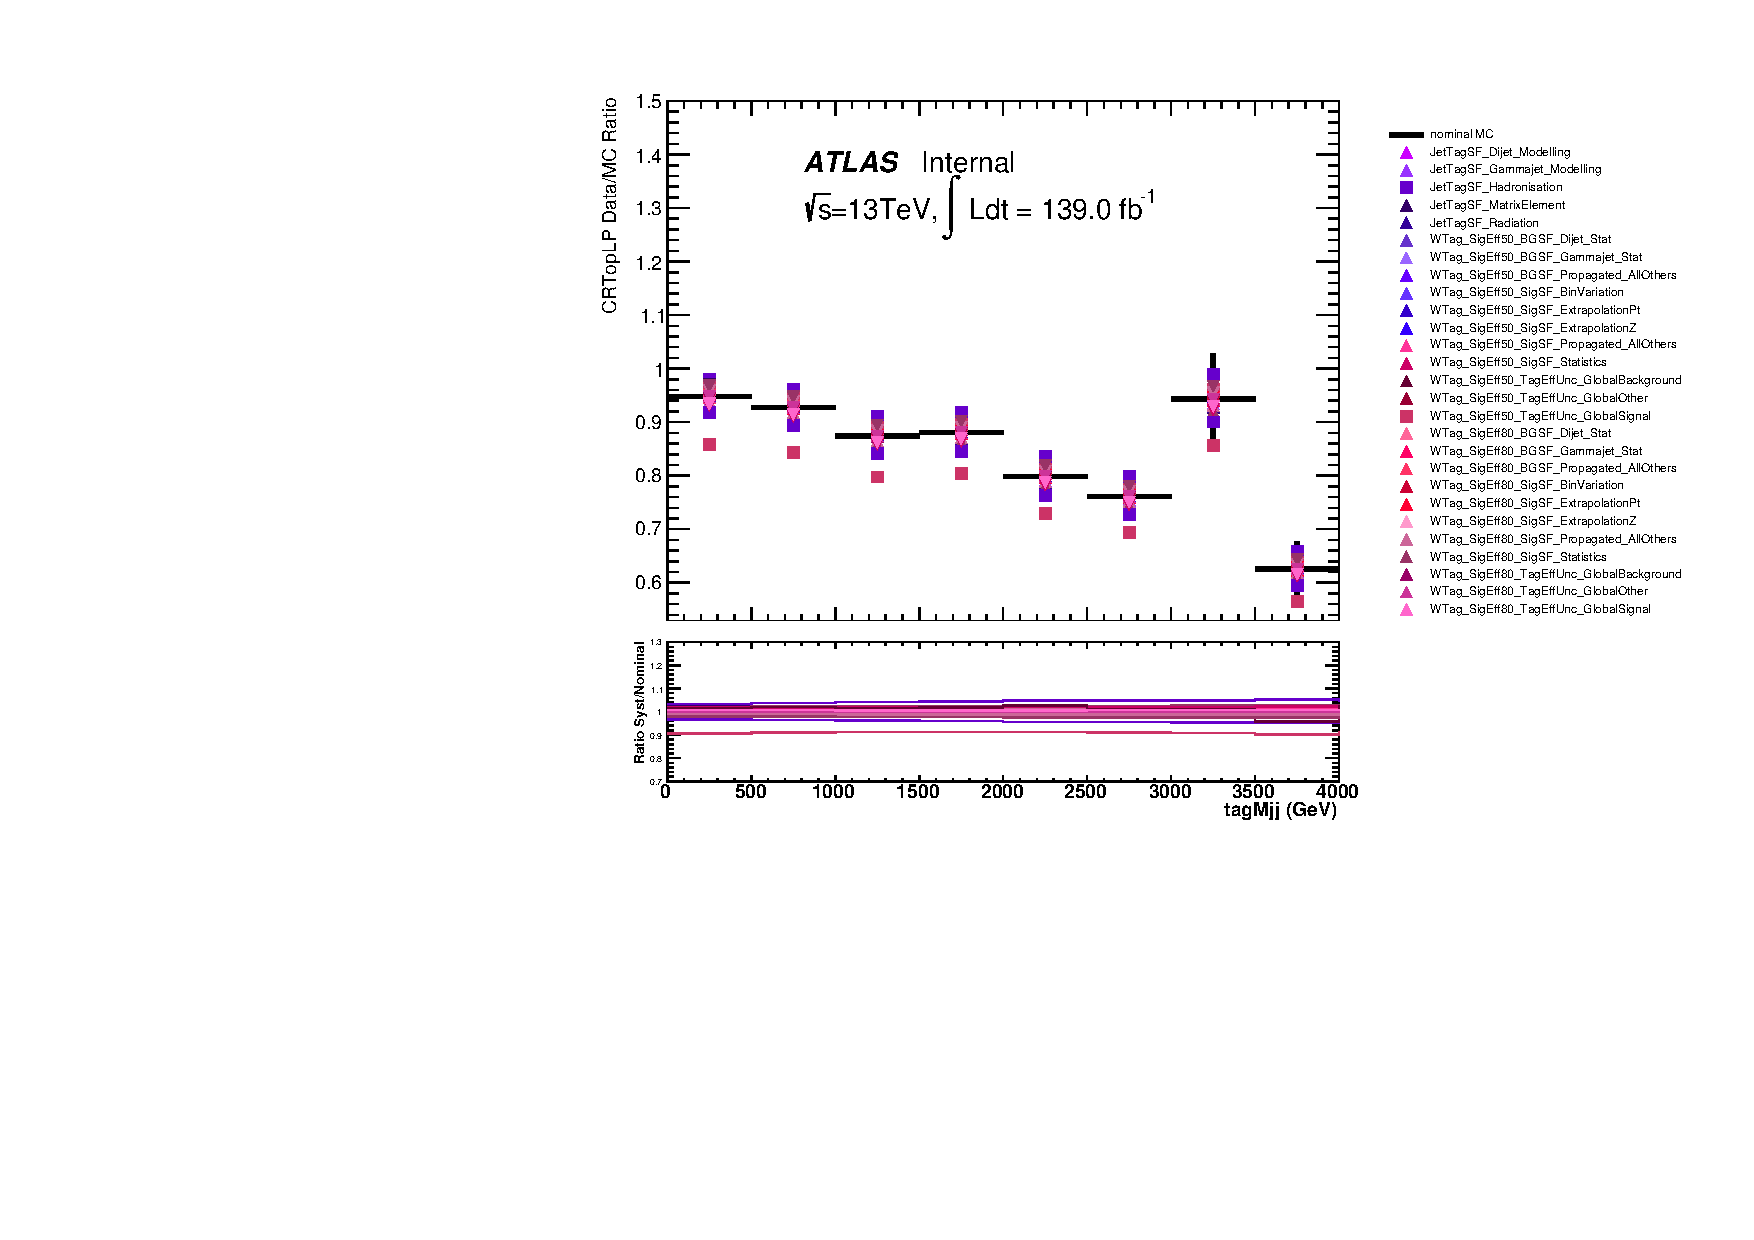
\includegraphics[width=\textwidth]{figures/1lep/VTaggerUnc/VTagCRTopLPtagMjj_SystBreakDown.pdf}
        \caption{Merged LP TopCR}
        \label{fig:MergedLPTopCR}
    \end{subfigure}
%    \hfill % This adds a bit of horizontal spacing between figures
    \begin{subfigure}[b]{0.3\textwidth}
        \centering
        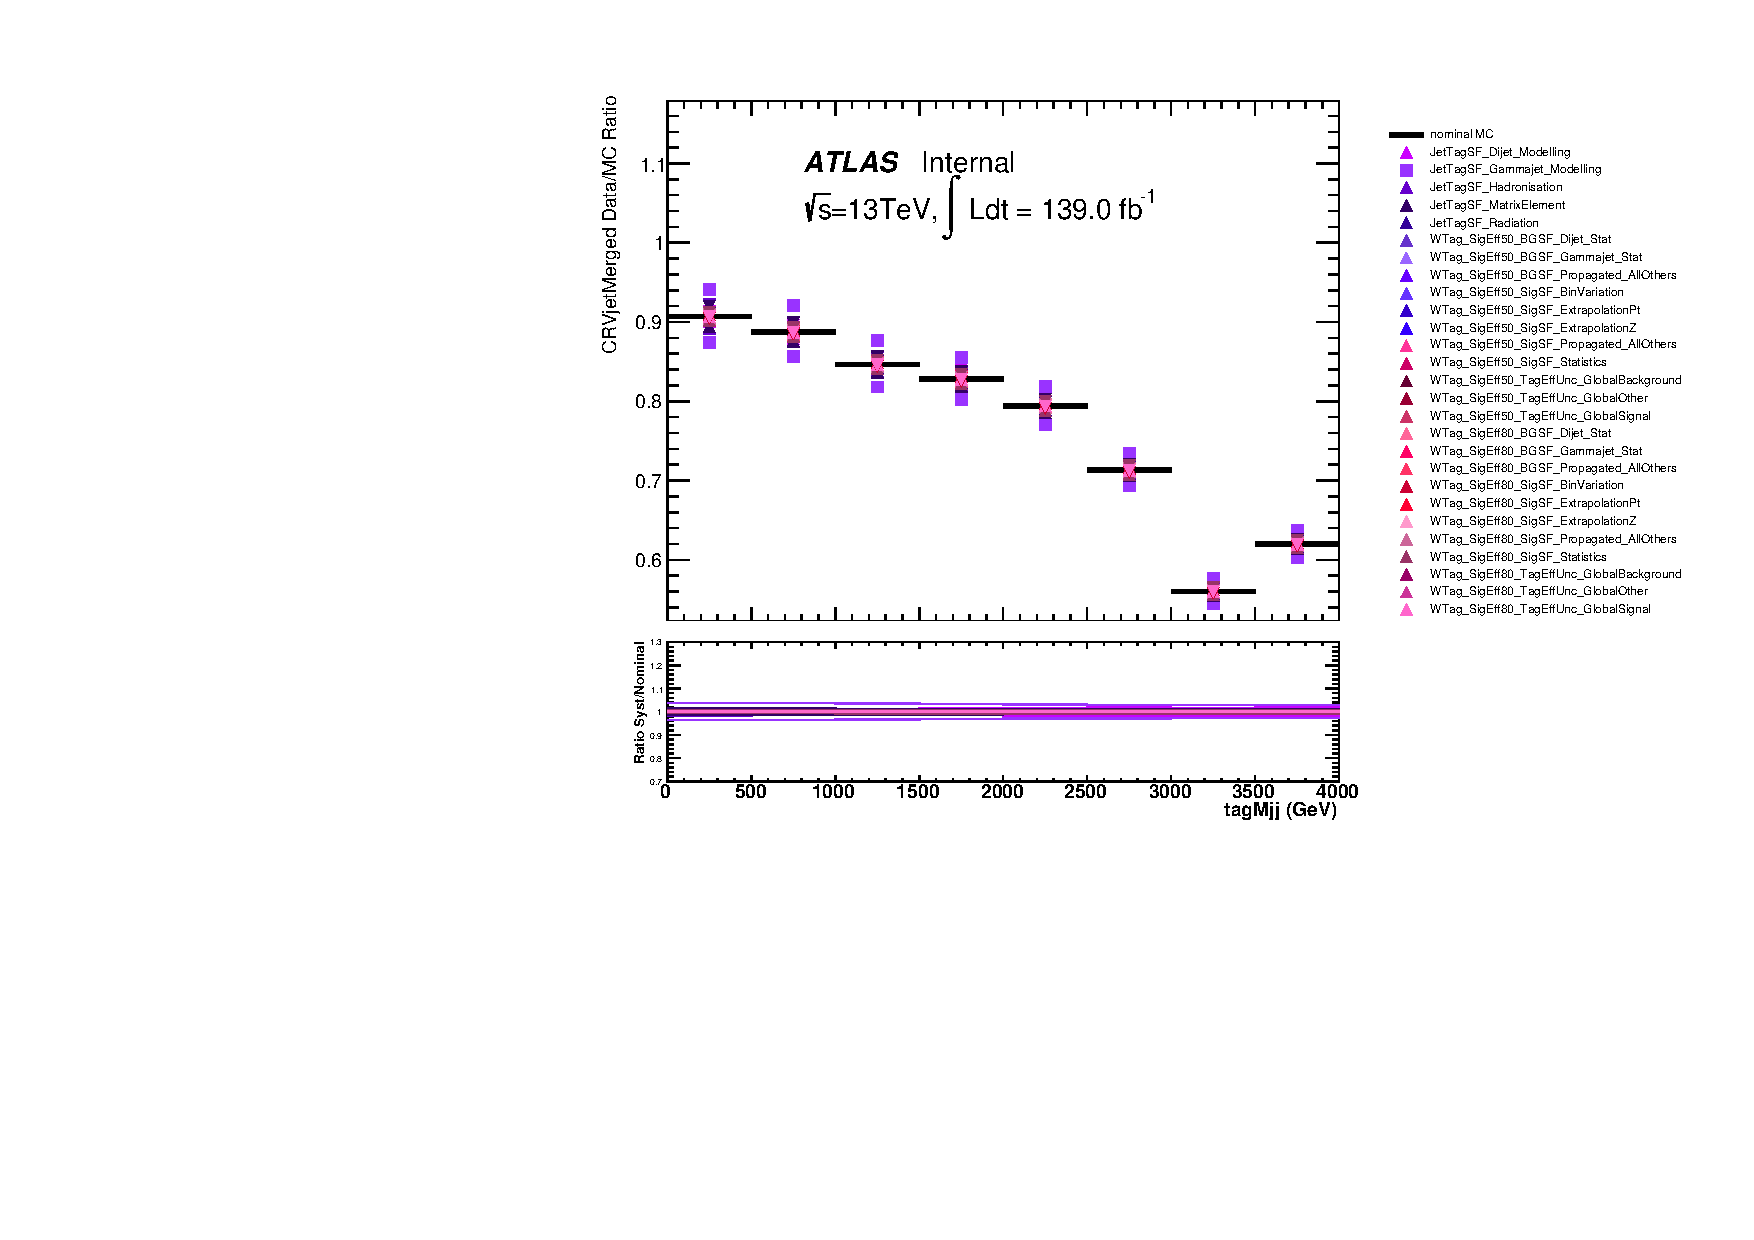
\includegraphics[width=\textwidth]{figures/1lep/VTaggerUnc/VTagCRVjetMergedtagMjj_SystBreakDown.pdf}
        \caption{Merged Wjets CR}
        \label{fig:MergedWjetsCR}
    \end{subfigure}
    \caption{Comparison of boson tagging scale factors in the 1-lepton channel.}
    \label{fig:1LepVTaggerUnc}
\end{figure}


%%%\begin{figure}[ht]
%%%    \centering
%%%        \subfigure[Merged CR]{\includegraphics[width=0.3\textwidth]{figures/2lep/taggerSF/0_MTagMerJets_SYS_CRVjet.pdf}}
%%%    	\subfigure[Merged HP SR]{\includegraphics[width=0.3\textwidth]{figures/2lep/taggerSF/0_MTagMerJets_SYS_SRVBS_HP.pdf}}
%%%        \subfigure[Merged LP SR]{\includegraphics[width=0.3\textwidth]{figures/2lep/taggerSF/0_MTagMerJets_SYS_SRVBS_LP.pdf}}
%%%        \caption{ Data/MC ratios as a function of the mass of the tagging jets in the 2-lepton channel. All tagger SF related uncertainties are plotted. The plots are before applying the re-weighting described in \ref{subsec:mjj_reweight_2lep}. All bins containing more than 5\% of signal are blinded in the SRs. } 
%%%    \label{fig:2lep_bkgUnc_BT}
%%%\end{figure}


%%%\begin{figure}[ht]
%%%    \centering
%%%        \subfigure[Merged HP TopCR]{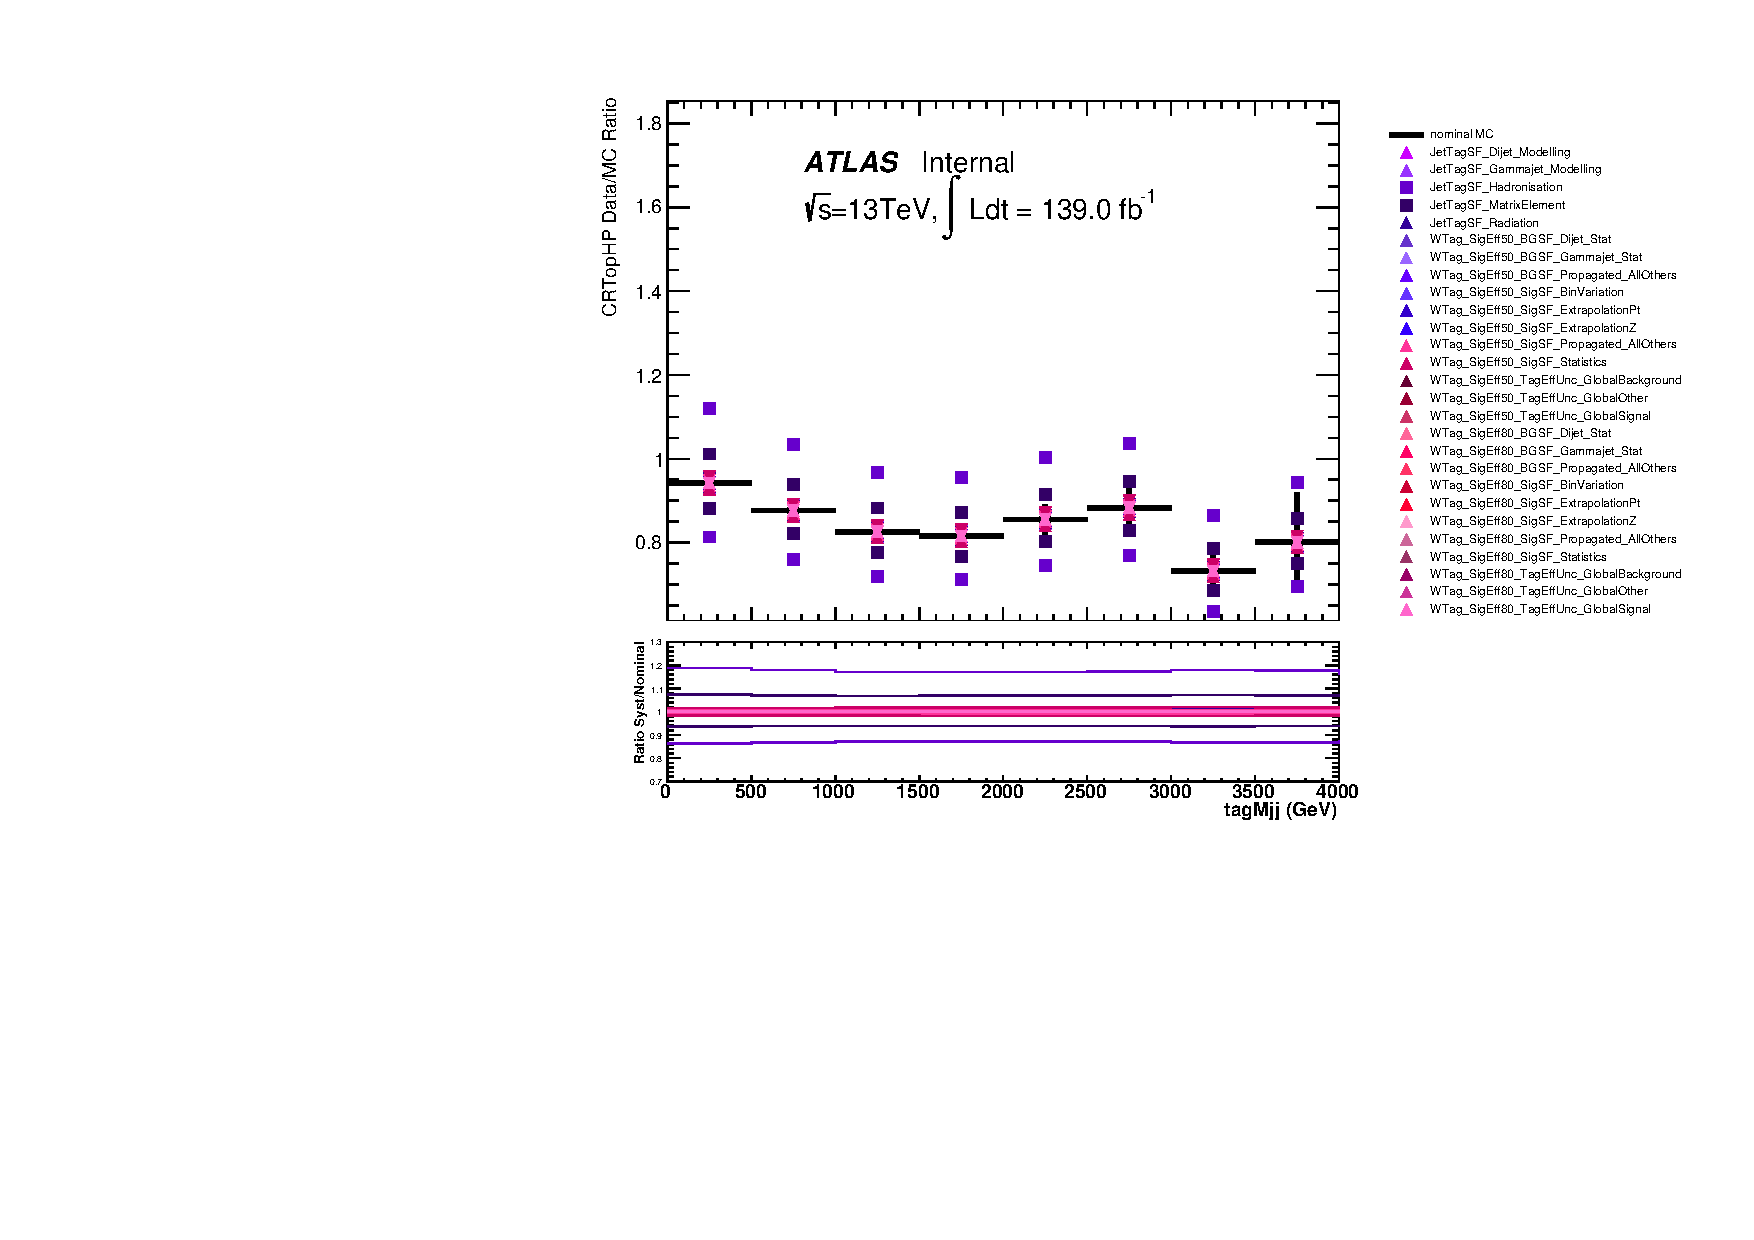
\includegraphics[width=0.3\textwidth]{figures/1lep/VTaggerUnc/VTagCRTopHPtagMjj_SystBreakDown.pdf}}
%%%    	\subfigure[Merged LP TopCR]{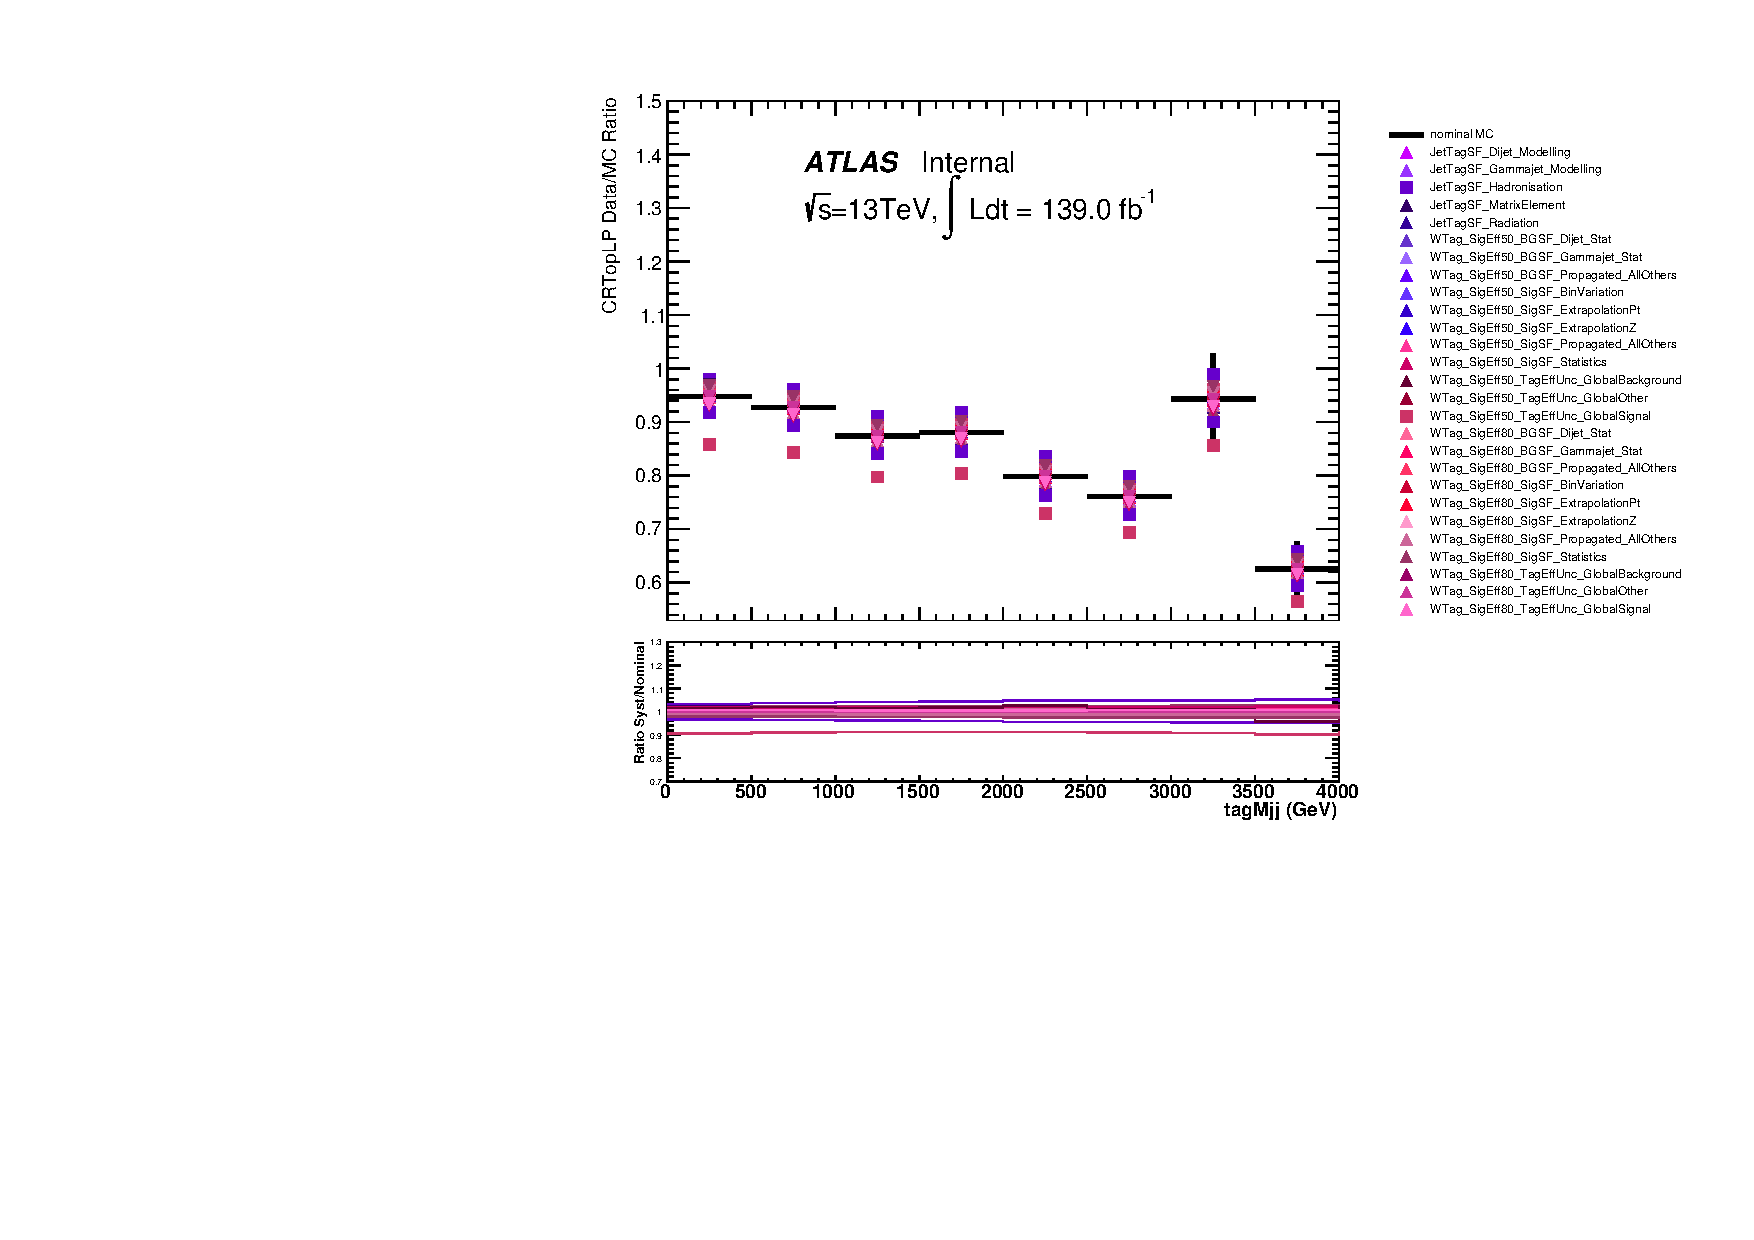
\includegraphics[width=0.3\textwidth]{figures/1lep/VTaggerUnc/VTagCRTopLPtagMjj_SystBreakDown.pdf}} 
%%%	\subfigure[Merged Wjets CR]{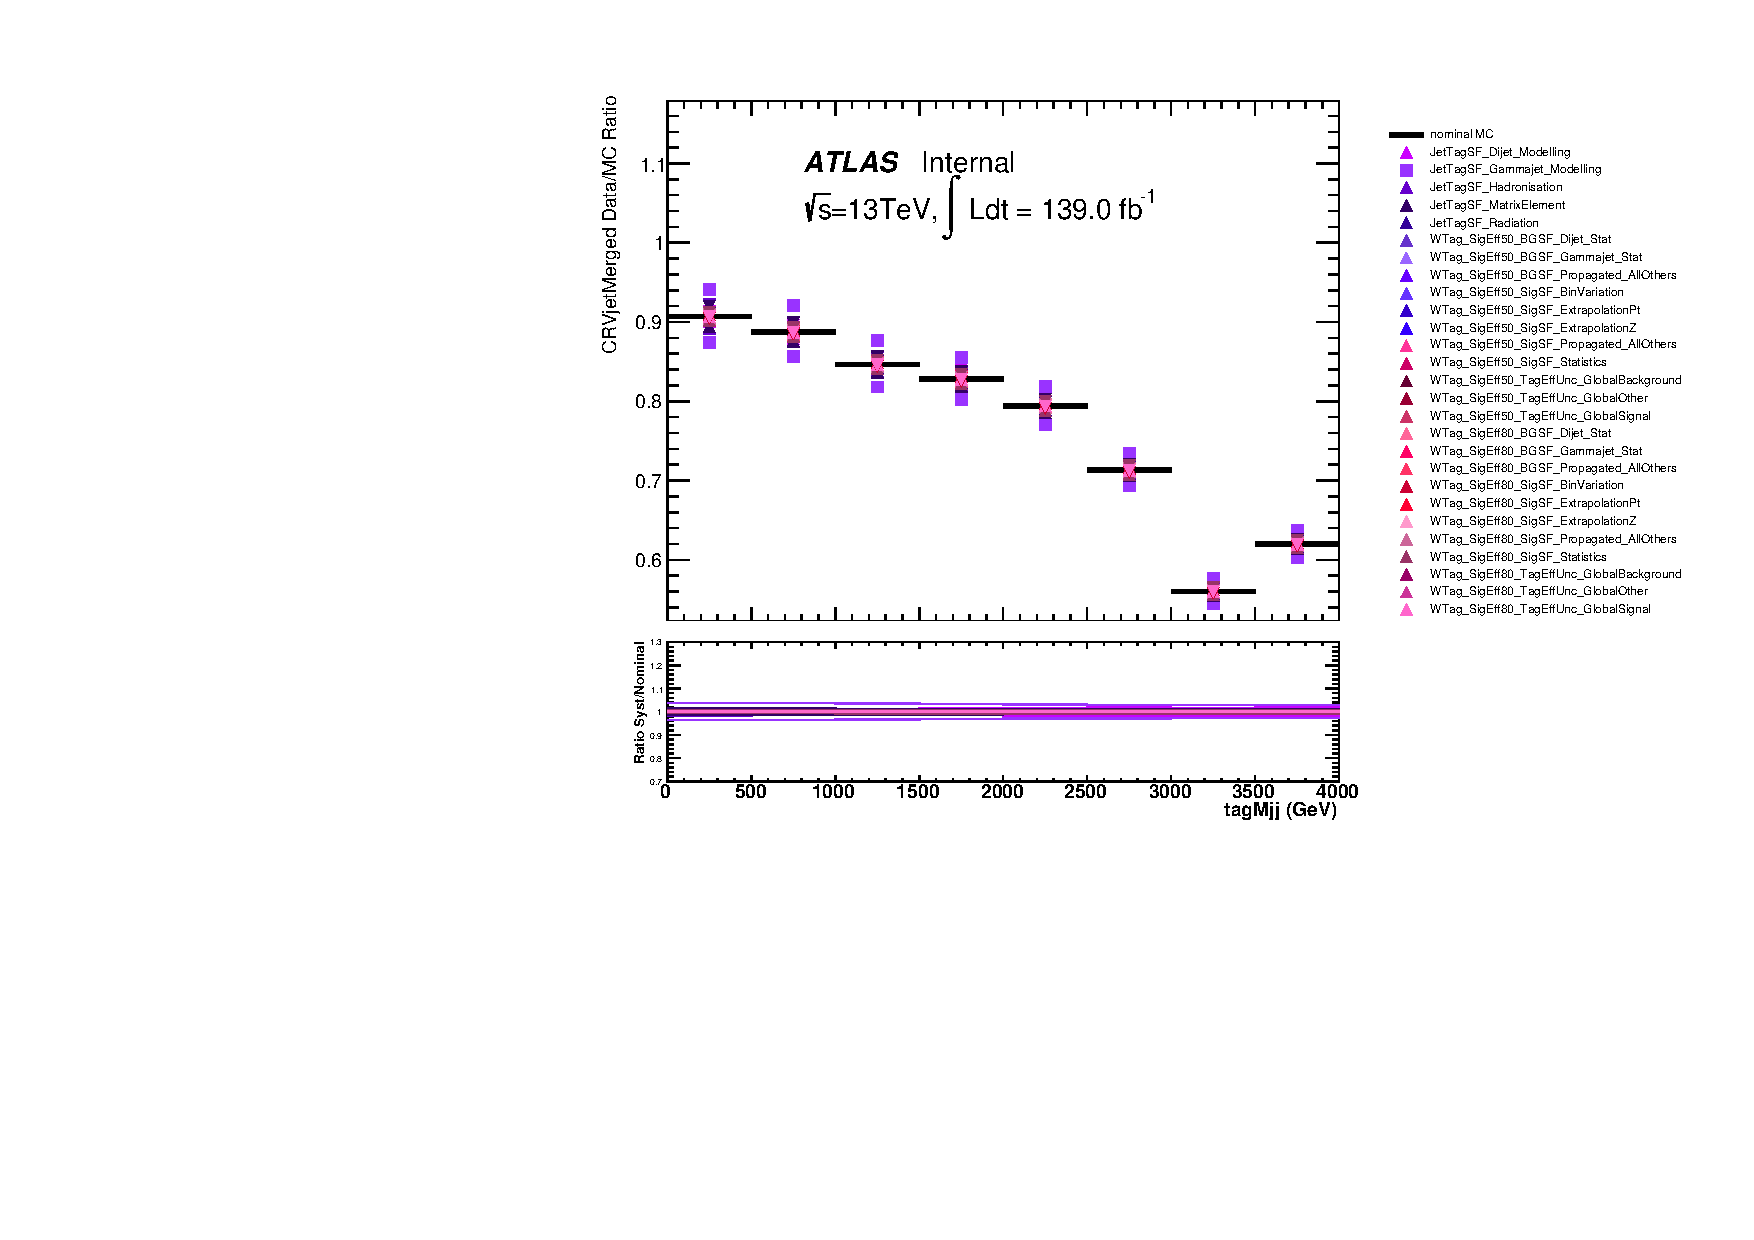
\includegraphics[width=0.3\textwidth]{figures/1lep/VTaggerUnc/VTagCRVjetMergedtagMjj_SystBreakDown.pdf}}
%%%        \caption{Comparison of boson tagging scale factors in the 1-lepton channel. } 
%%%    \label{fig:1LepVTaggerUnc}
%%%\end{figure}


%%%\begin{figure}[ht]
%%%    \centering
%%%      	\subfigure[signal: Merged CR]{\includegraphics[width=0.3\textwidth]{figures/0lep/systematics/systs/merged/plots/systvtagSigsig_RNN_CRVjet_Mer.pdf}}
%%%    	\subfigure[signal: Merged HP SR]{\includegraphics[width=0.3\textwidth]{figures/0lep/systematics/systs/merged/plots/systvtagSigsig_RNN_SRVBS_HP.pdf}}
%%%        \subfigure[signal: Merged LP SR]{\includegraphics[width=0.3\textwidth]{figures/0lep/systematics/systs/merged/plots/systvtagSigsig_RNN_SRVBS_LP.pdf}}\\
%%%      	\subfigure[background: Merged CR]{\includegraphics[width=0.3\textwidth]{figures/0lep/systematics/systs/merged/plots/systvtagBkgWjets_nom_Zjets_nom_diboson_stop_ttbar_nom_RNN_CRVjet_Mer.pdf}}
%%%    	\subfigure[background: Merged HP SR]{\includegraphics[width=0.3\textwidth]{figures/0lep/systematics/systs/merged/plots/systvtagBkgWjets_nom_Zjets_nom_diboson_stop_ttbar_nom_RNN_SRVBS_HP.pdf}}
%%%        \subfigure[background: Merged LP SR]{\includegraphics[width=0.3\textwidth]{figures/0lep/systematics/systs/merged/plots/systvtagBkgWjets_nom_Zjets_nom_diboson_stop_ttbar_nom_RNN_SRVBS_HP.pdf}}\\
%%%        \caption{Effect of all tagger SF related uncertainties in the 0-lepton channel on the signal MC and on all background MCs together.} 
%%%    \label{fig:0LepVTaggerUnc}
%%%\end{figure}



%%%
\subsection{Quark/Gluon jets uncertainty}
%\subsubsection{Quark/Gluon jets uncertainty}
\label{subsec:bkg_uncer_qg}

Jet flavor response and composition uncertainties consider the different jet responses to quark- and gluon-initiated jets. 
The response uncertainties are centrally derived from dijet events using alternative MC samples, specifically Pythia 8 and Herwig++. 
For flavor composition, uncertainties are typically assumed based on a 50/50 quark/gluon mix, with a conservative (100\%) uncertainty. 
However, in VBS topologies, which tend to be quark-enriched, such uncertainties can limit measurement sensitivity. 
To mitigate this, we study the gluon fraction within our analysis phase-space. 
This allows us to rederive jet flavor-related uncertainties using custom gluon fractions, thus potentially reducing these uncertainties.

The estimation of the gluon fraction across various analysis regions and samples is performed as a function of the small-\(R\) jet \(\pt\) and \(\eta\). This is achieved by utilizing truth parton label information to discern the quantity of quarks and gluons. For the purpose of quark estimation, all jets are considered in the denominator, with the exception of those initiated by b-quarks.

The gluon fraction for each analysis region and across various samples is calculated based on the small-$R$ jet $\pt$ and $\eta$. 
This estimation utilizes truth parton label information to determine the number of quarks and gluons. 
For the purpose of quark estimation, all jets except those initiated by $b$-quarks are considered in the denominator.

Two-dimensional histograms, representing the gluon fraction as a function of jet $\pt$ and $\eta$, serve as inputs for recalculating jet flavor and composition uncertainties. Each MC sample is associated with a single input file. 
The gluon fraction for a specific ($\pt$, $\eta$) bin is determined by aggregating data across all regions, according to the nominal approach.

To account for the uncertainty in the gluon fraction, additional inputs are utilized. The uncertainty for a particular ($\pt$, $\eta$) bin, $\sigma_{gfrac}$, is calculated as follows:
\[
\sigma_{gfrac} = \sqrt{\sigma_{region}^{2} + \sigma_{gen}^{2}}
\]
Here, \(\sigma_{region}\) represents the maximal deviation in gluon fraction between the nominal and any analysis region. Meanwhile, \(\sigma_{gen}\) denotes the generator uncertainty, obtained from comparing alternative Pythia 8 and Herwig++ MC samples.


The inputs for the gluon fraction and their corresponding uncertainties in the \olep channel are illustrated in Figures \ref{fig:QGFracInputs2D1Lep} and \ref{fig:QGFracErrorInputs2D1Lep}, respectively. 
Comparison between old flavor uncertainties and newly derived flavor uncertainties is shown is Figure \ref{fig:1LepFlavorVarOldNew}. It is evident from this comparison that flavor composition uncertainties, in general, are reduced.


%%%%%%%%
%%%The jet flavor response and composition uncertainties account for the different jet responses to quark- and gluon-initiated jets. The flavor response uncertainties are derived centrally from dijet events using alternative (Pythia 8 and Herwig++) Monte Carlo. Flavor composition uncertainties are usually derived assuming a 50/50 quark/gluon composition with a very conservative (100\%) uncertainty. In VBS topologies where quark enriched regions are expected such uncertainties can limit the sensitivity of the measurement. In order to reduce such uncertainties, the gluon fraction in our analysis phase-space is studied and jet flavor related uncertainties are rederived using custom gluon fractions. %anastasia; Maybe add formulas for jet flavour composition and jet flavour response from dimitris lectures
%%%
%%%The gluon fraction in each of the analysis regions and for the different analysis samples is estimated as a function of the small-$R$ jet $\pt$ and $\eta$. Truth parton label information is used in order to estimate the number of quarks and gluons.  All jets except b-quark-initiated jets are included in the denominator for the quark estimation. 
%%%
%%%In Figures \ref{fig:2lep_gfrac_pt} and  \ref{fig:2lep_gfrac_eta} a comparison of the gluon fraction between the different analysis regions for the 2-lepton channel main MC samples is plotted as a function of $\pt$ and $\eta$ respectively. A clear $\pt$ and $\eta$ dependence of the gluon fraction is noticed.
%%%
%%%2D histograms of the gluon fraction as a function of  $\pt$ and $\eta$ are used as inputs to recalculate the jet flavor and composition uncertainties. A single input file per MC sample is used. The gluon fraction for a given bin in $\pt$ and $\eta$ is given after summing up all regions (nominal approach). This approach is very similar to computing the average gluon fraction between regions as shown by comparing the red and black histograms of Figure \ref{fig:2lep_gfrac_eta}. Additional inputs to describe the uncertainty on the gluon fraction are also provided. The uncertainty in a given $\pt,\eta$ bin is given by: $$ \sigma_{gfrac} = \sqrt{\sigma_{region}^{2}+\sigma_{gen}^{2} } $$ where $\sigma_{region}$ is the maximum difference in gluon fraction between nominal and an analysis region, $\sigma_{gen}$ is the generator uncertainty derived using alternative Pythia 8 and Herwig MC samples. In Figures \ref{fig:2lep_gfrac_alt_pt} and  \ref{fig:2lep_gfrac_alt_eta} a comparison of the nominal gluon fraction and gluon fraction as calculated by using alternative samples is plotted for the main background sources in the 2-lepton channel. For cases where alternative samples are not available (e.g for Signal) the region only uncertainties are considered. %anastasia; maybe comment that the region uncertainties are usually much larger than the ones coming from alternative samples.
%%%
%%%The gluon fraction inputs and their corresponding uncertainties for the 2-lepton channel are plotted in Figures  \ref{fig:2lep_gfrac_2D} and  \ref{fig:2lep_gfrac_err_2D} respectively. Similar plots for the 0- and 1-lepton channels can be found in appendix \ref{app:QGfraction}. 

%%%%%%%%%%%%%


\begin{figure}[p]
    \centering
    \begin{subfigure}[b]{0.3\textwidth}
        \centering
        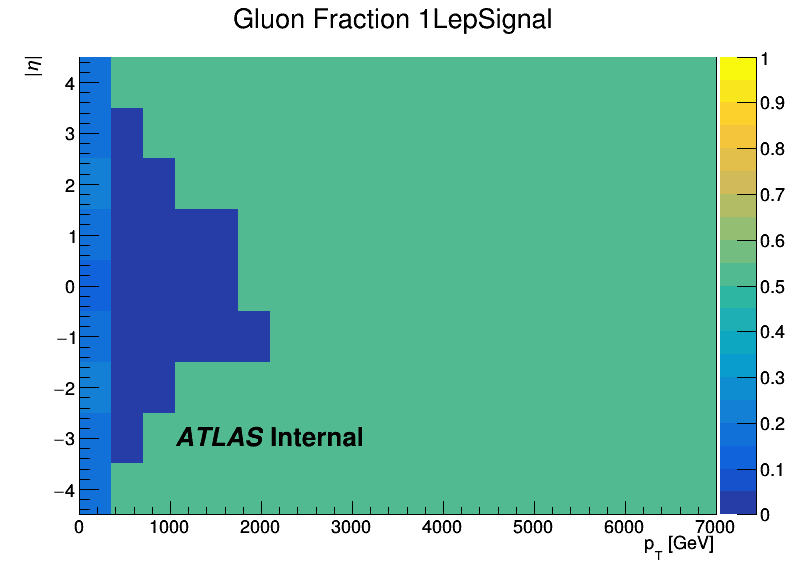
\includegraphics[width=\textwidth]{figures/QGfrac/GluonFrac2D_1LepSignal.png}
        \caption{Signal samples}
        \label{fig:GluonFracSignal}
    \end{subfigure}
    \hfill
    \begin{subfigure}[b]{0.3\textwidth}
        \centering
        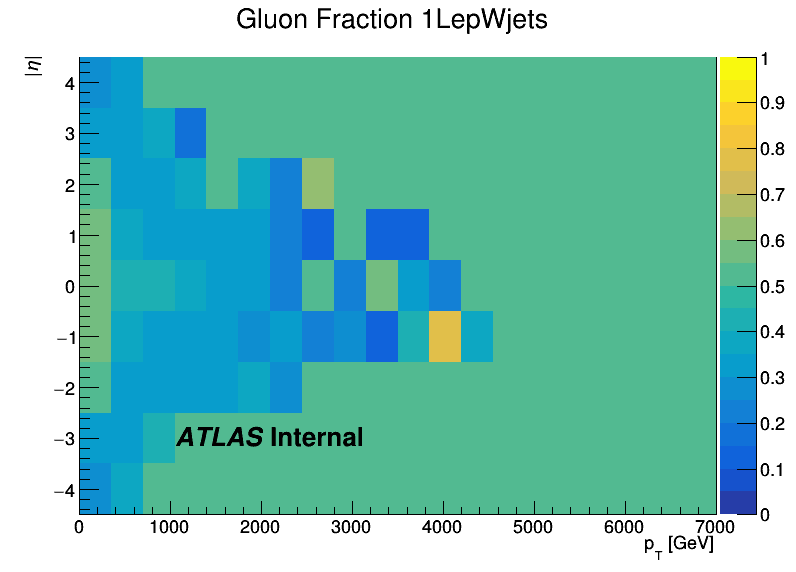
\includegraphics[width=\textwidth]{figures/QGfrac/GluonFrac2D_1LepWjets.png}
        \caption{\Wjets samples}
        \label{fig:GluonFracWjets}
    \end{subfigure}
    \hfill
    \begin{subfigure}[b]{0.3\textwidth}
        \centering
        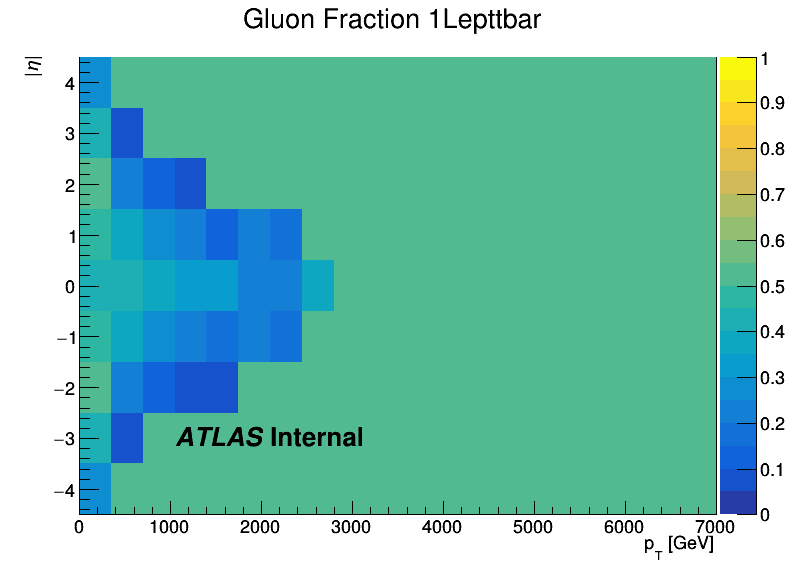
\includegraphics[width=\textwidth]{figures/QGfrac/GluonFrac2D_1Lepttbar.png}
        \caption{ttbar samples}
        \label{fig:GluonFracttbar}
    \end{subfigure}

    \bigskip

    \begin{subfigure}[b]{0.3\textwidth}
        \centering
        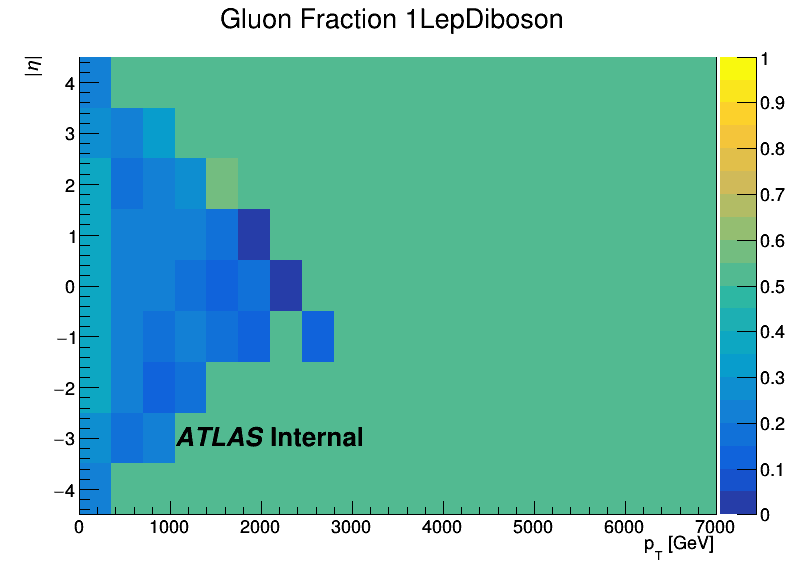
\includegraphics[width=\textwidth]{figures/QGfrac/GluonFrac2D_1LepDiboson.png}
        \caption{Diboson samples}
        \label{fig:GluonFracDiboson}
    \end{subfigure}
%    \hfill
    \begin{subfigure}[b]{0.3\textwidth}
        \centering
        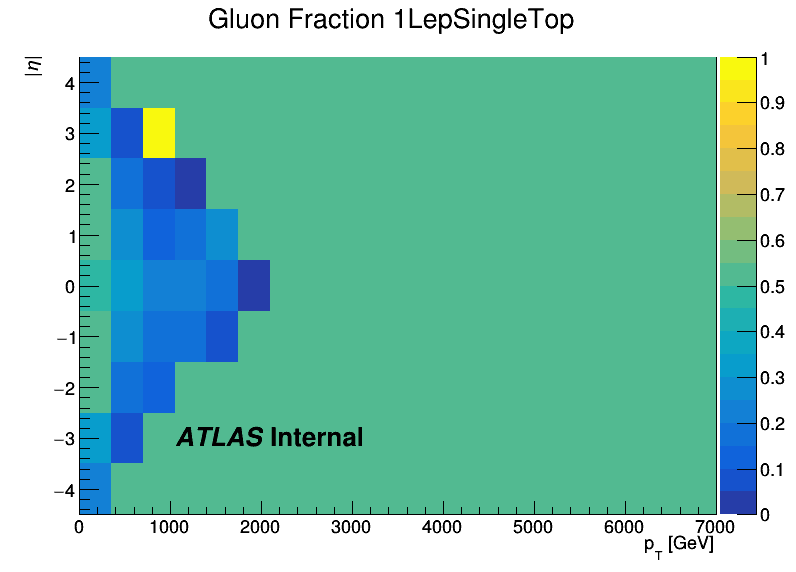
\includegraphics[width=\textwidth]{figures/QGfrac/GluonFrac2D_1LepSingleTop.png}
        \caption{Single top samples}
        \label{fig:GluonFracSingleTop}
    \end{subfigure}
    \hfill

    \caption{Gluon fraction inputs used to calculate jet uncertainties for the 1 lepton channel.}
    \label{fig:QGFracInputs2D1Lep}
\end{figure}


\begin{figure}[p]
    \centering
    \begin{subfigure}[b]{0.3\textwidth}
        \centering
        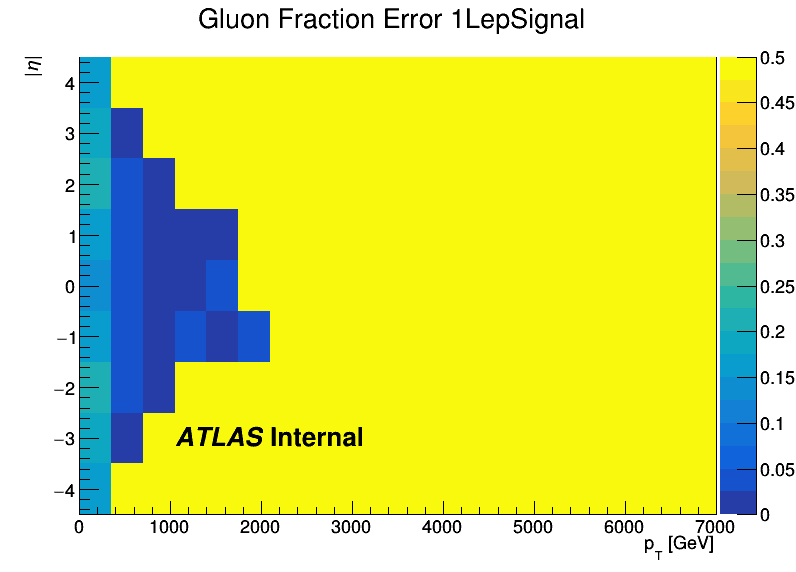
\includegraphics[width=\textwidth]{figures/QGfrac/GluonFracError2D_1LepSignal.png}
        \caption{Signal samples}
        \label{fig:GluonFracErrorSignal}
    \end{subfigure}
    \hfill
    \begin{subfigure}[b]{0.3\textwidth}
        \centering
        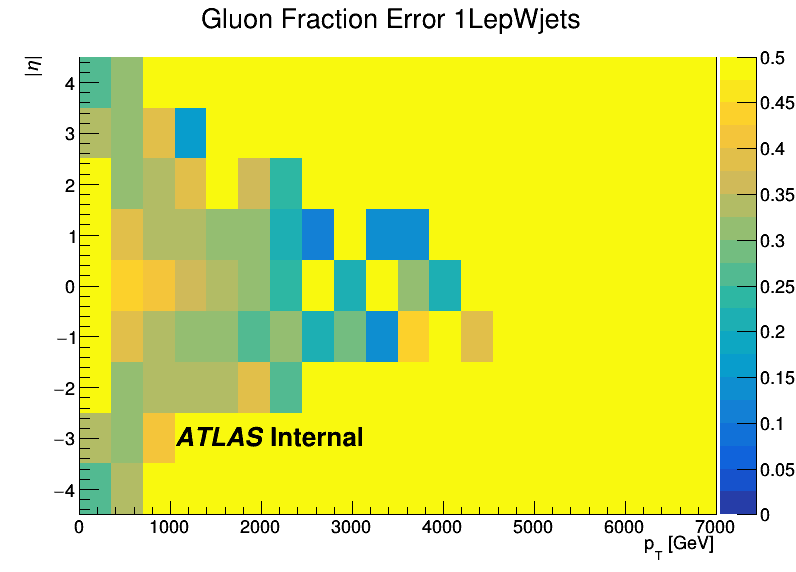
\includegraphics[width=\textwidth]{figures/QGfrac/GluonFracError2D_1LepWjets.png}
        \caption{\Wjets samples}
        \label{fig:GluonFracErrorWjets}
    \end{subfigure}
    \hfill
    \begin{subfigure}[b]{0.3\textwidth}
        \centering
        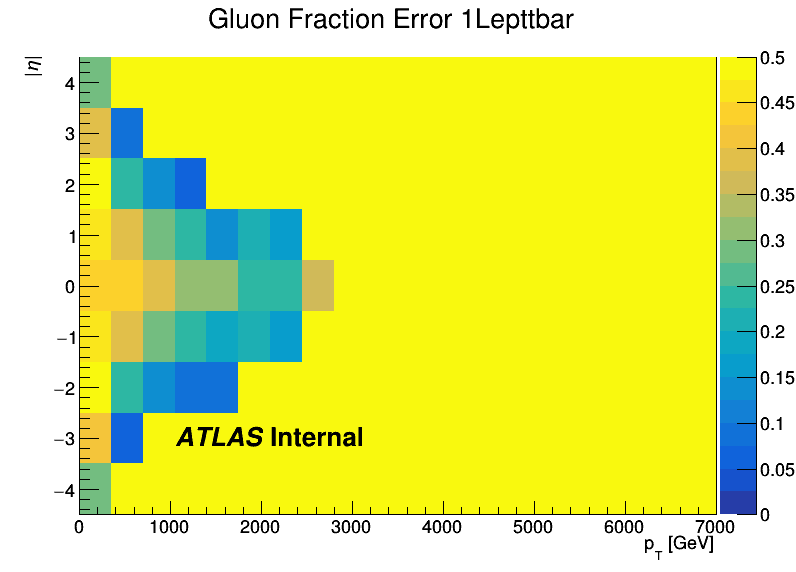
\includegraphics[width=\textwidth]{figures/QGfrac/GluonFracError2D_1Lepttbar.png}
        \caption{ttbar samples}
        \label{fig:GluonFracErrorttbar}
    \end{subfigure}

    \bigskip

    \begin{subfigure}[b]{0.3\textwidth}
        \centering
        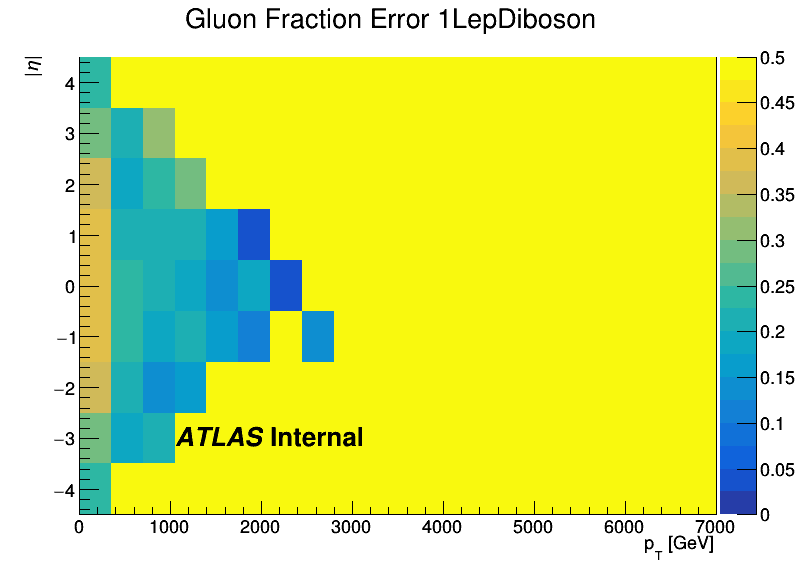
\includegraphics[width=\textwidth]{figures/QGfrac/GluonFracError2D_1LepDiboson.png}
        \caption{Diboson samples}
        \label{fig:GluonFracErrorDiboson}
    \end{subfigure}
%    \hfill
    \begin{subfigure}[b]{0.3\textwidth}
        \centering
        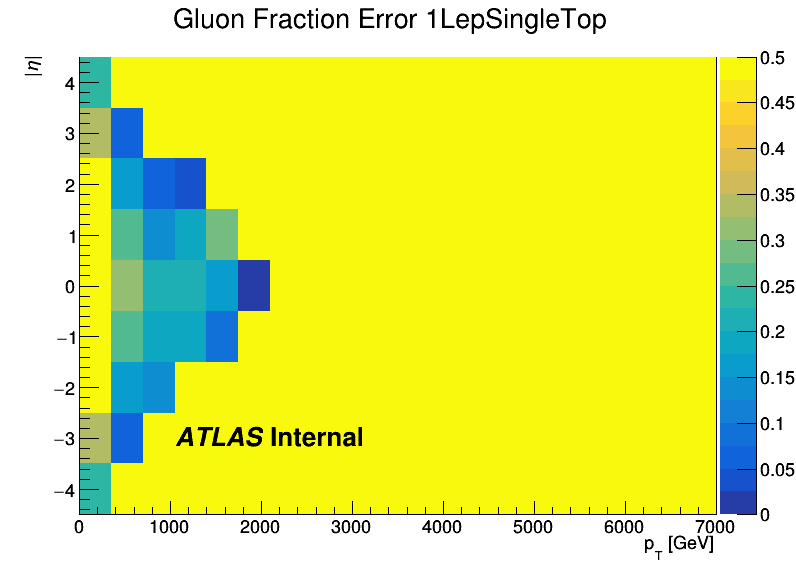
\includegraphics[width=\textwidth]{figures/QGfrac/GluonFracError2D_1LepSingleTop.png}
        \caption{Single top samples}
        \label{fig:GluonFracErrorSingleTop}
    \end{subfigure}
    \hfill

    \caption{Gluon fraction error inputs used to calculate jet uncertainties for the 1 lepton channel.}
    \label{fig:QGFracErrorInputs2D1Lep}
\end{figure}


\begin{figure}[ht]
    \centering
    \begin{subfigure}[b]{0.4\textwidth}
        \centering
        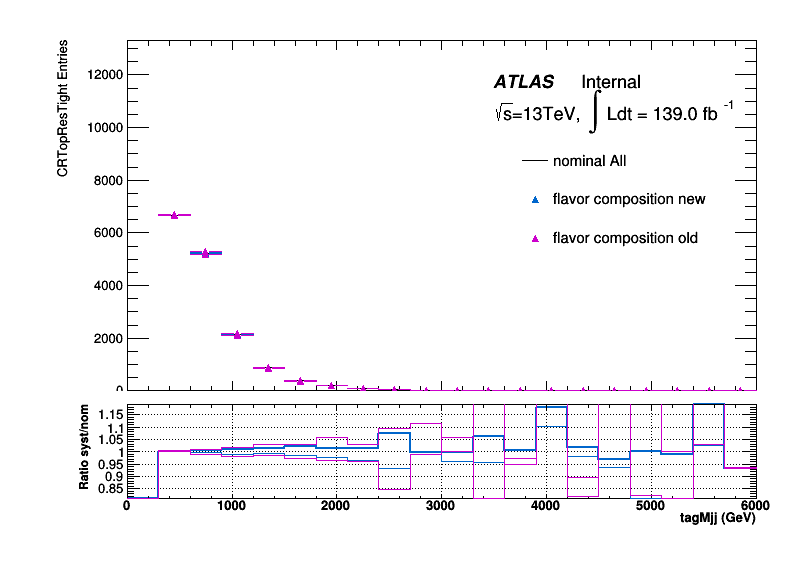
\includegraphics[width=\textwidth]{figures/1lep/FlavorVar/SystFCompCRTopResTight_All_tagMjj.png}
        \caption{Resolved TopCR Flavour Composition}
        \label{fig:ResolvedTopCRFlavourComposition}
    \end{subfigure}
    \quad % This adds some spacing between the figures in the same row
    \begin{subfigure}[b]{0.4\textwidth}
        \centering
        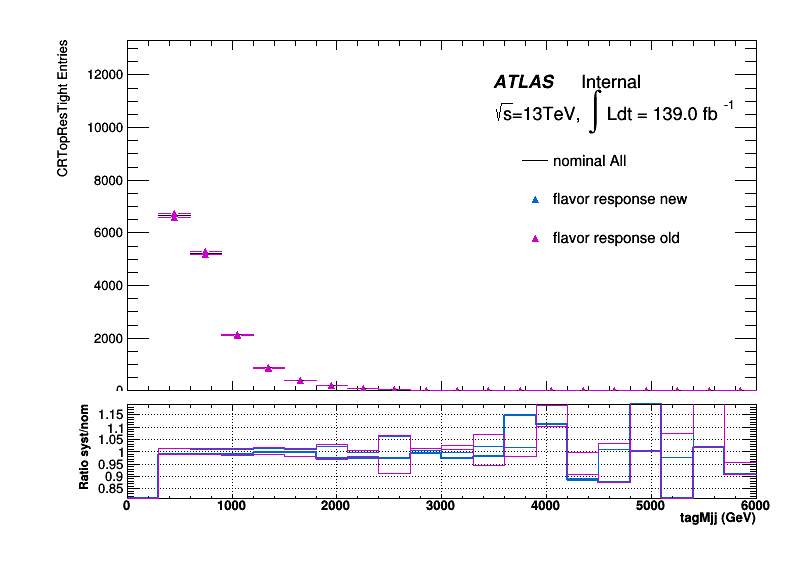
\includegraphics[width=\textwidth]{figures/1lep/FlavorVar/SystFResCRTopResTight_All_tagMjj.png}
        \caption{Resolved TopCR Flavour Response}
        \label{fig:ResolvedTopCRFlavourResponse}
    \end{subfigure}

    \bigskip % This adds extra vertical spacing between the rows of figures

    \begin{subfigure}[b]{0.4\textwidth}
        \centering
        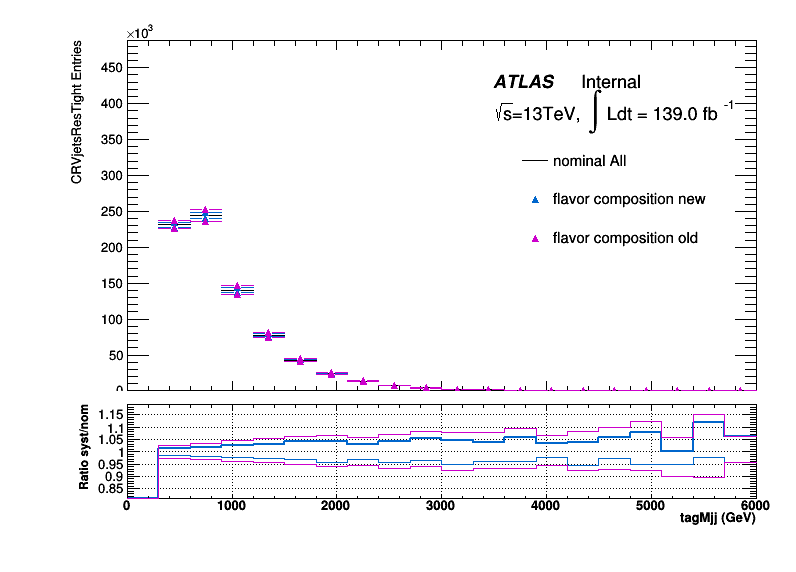
\includegraphics[width=\textwidth]{figures/1lep/FlavorVar/SystFCompCRVjetsResTight_All_tagMjj.png}
        \caption{Resolved WjetsCR Flavour Composition}
        \label{fig:ResolvedWjetsCRFlavourComposition}
    \end{subfigure}
    \quad % This adds some spacing between the figures in the same row
    \begin{subfigure}[b]{0.4\textwidth}
        \centering
        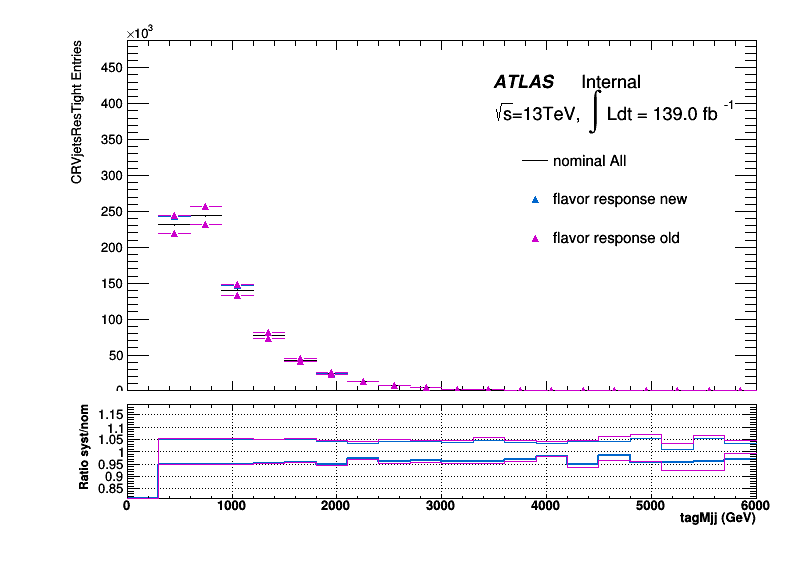
\includegraphics[width=\textwidth]{figures/1lep/FlavorVar/SystFResCRVjetsResTight_All_tagMjj.png}
        \caption{Resolved WjetsCR Flavour Response}
        \label{fig:ResolvedWjetsCRFlavourResponse}
    \end{subfigure}

    \caption{Comparison between old flavor uncertainties and newly derived flavor uncertainties.}
    \label{fig:1LepFlavorVarOldNew}
\end{figure}


% Flavour Variations for mc16a 1lep
%%%\begin{figure}[ht]
%%%    \centering
%%%        \subfigure[Resolved TopCR Flavour Composition]{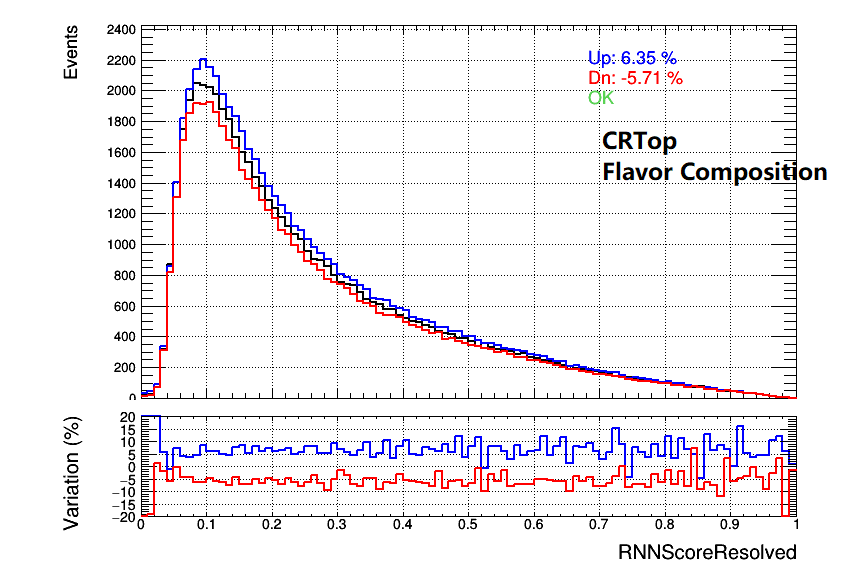
\includegraphics[width=0.4\textwidth]{figures/1lep/FlavorVar/C_0ptag2pjet_0ptv_CRTop_RNNScoreResolved_SysJET_Flavor_Composition.png}}
%%%        \subfigure[Resolved TopCR Flavour Response]{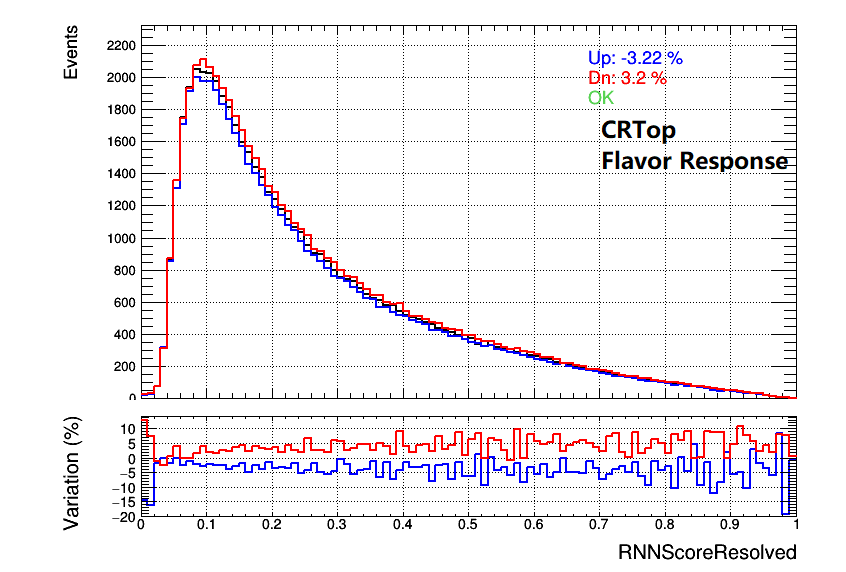
\includegraphics[width=0.4\textwidth]{figures/1lep/FlavorVar/C_0ptag2pjet_0ptv_CRTop_RNNScoreResolved_SysJET_Flavor_Response.png}}\\
%%%
%%%        \subfigure[Resolved WjetCR Flavour Composition]{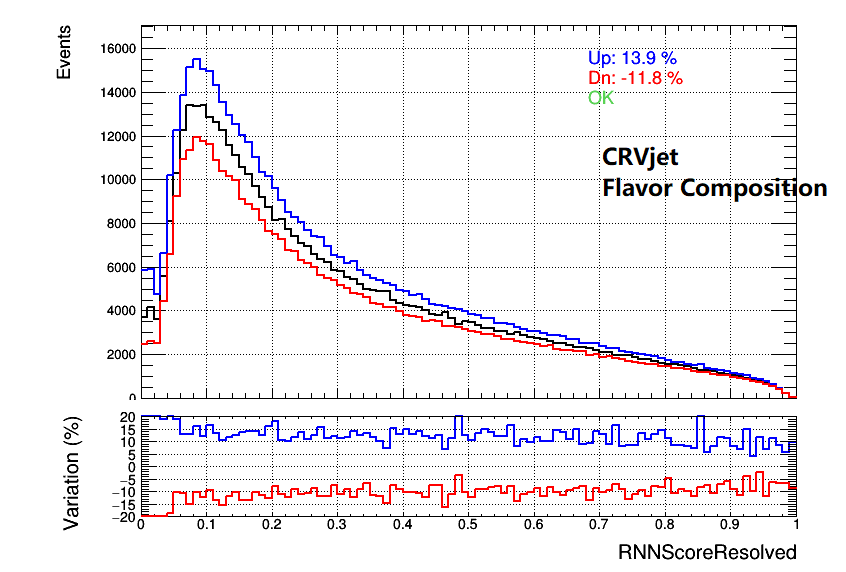
\includegraphics[width=0.4\textwidth]{figures/1lep/FlavorVar/C_0ptag2pjet_0ptv_CRVjet_RNNScoreResolved_SysJET_Flavor_Composition.png}}
%%%	\subfigure[Resolved WjetCR Flavour Reponse]{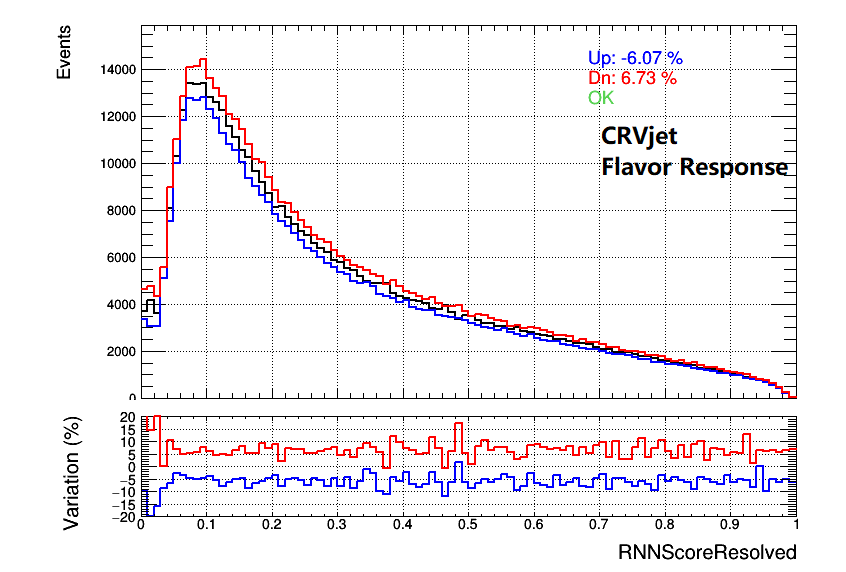
\includegraphics[width=0.4\textwidth]{figures/1lep/FlavorVar/C_0ptag2pjet_0ptv_CRVjet_RNNScoreResolved_SysJET_Flavor_Response.png}}
%%%
%%%        \caption{Impact of Flavour related variations on 1lepton resolved control regions. MC16A events are shown.}
%%%    \label{fig:1LepFlavorVariation}
%%%\end{figure}
%\begin{figure}[ht]
%    \centering
%        \subfigure[Resolved TopCR Flavour Composition]{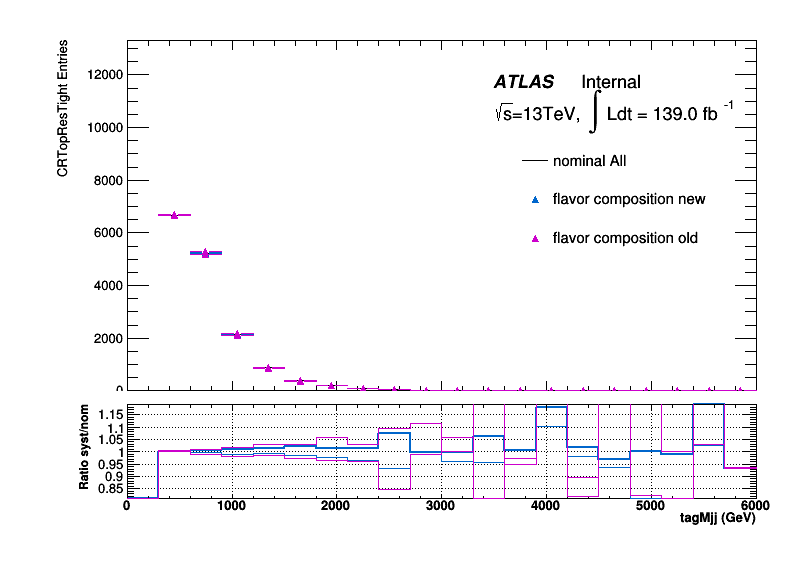
\includegraphics[width=0.4\textwidth]{figures/1lep/FlavorVar/SystFCompCRTopResTight_All_tagMjj.png}}
%        \subfigure[Resolved TopCR Flavour Response]{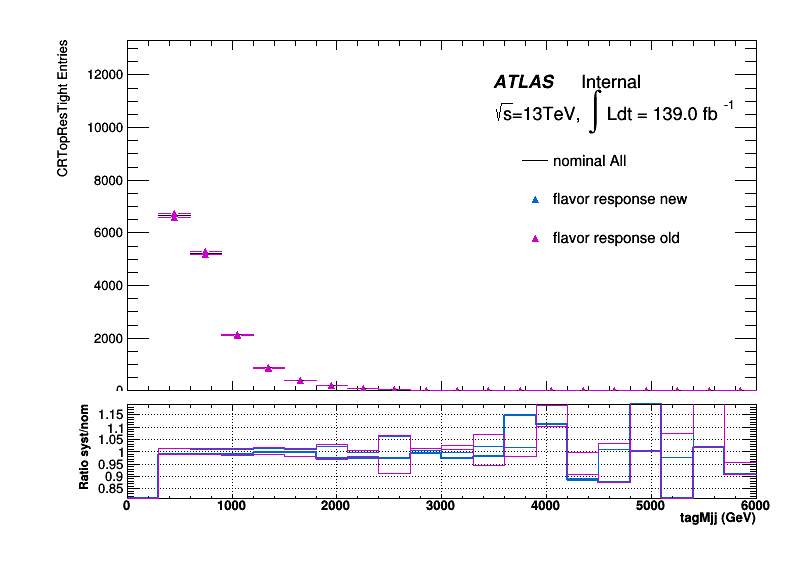
\includegraphics[width=0.4\textwidth]{figures/1lep/FlavorVar/SystFResCRTopResTight_All_tagMjj.png}} \\
%        \subfigure[Resolved WjetsCR Flavour Composition]{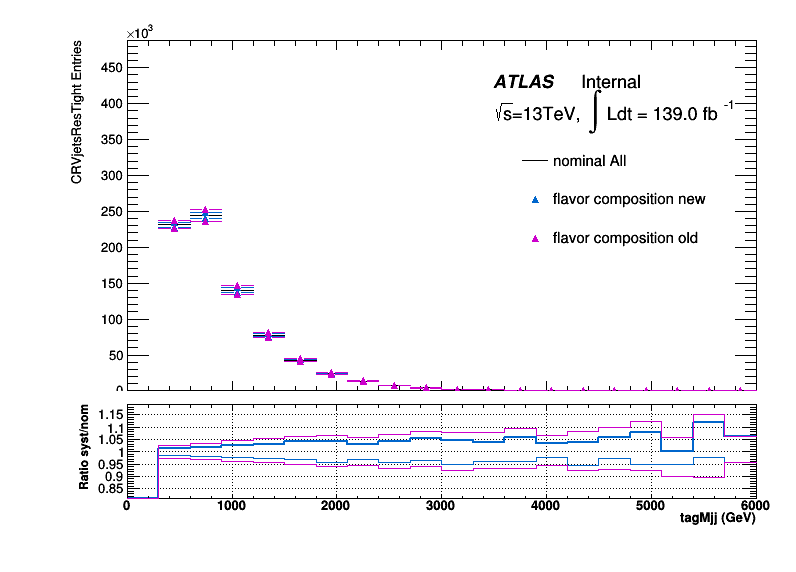
\includegraphics[width=0.4\textwidth]{figures/1lep/FlavorVar/SystFCompCRVjetsResTight_All_tagMjj.png}}
%        \subfigure[Resolved WjetsCR Flavour Reponse]{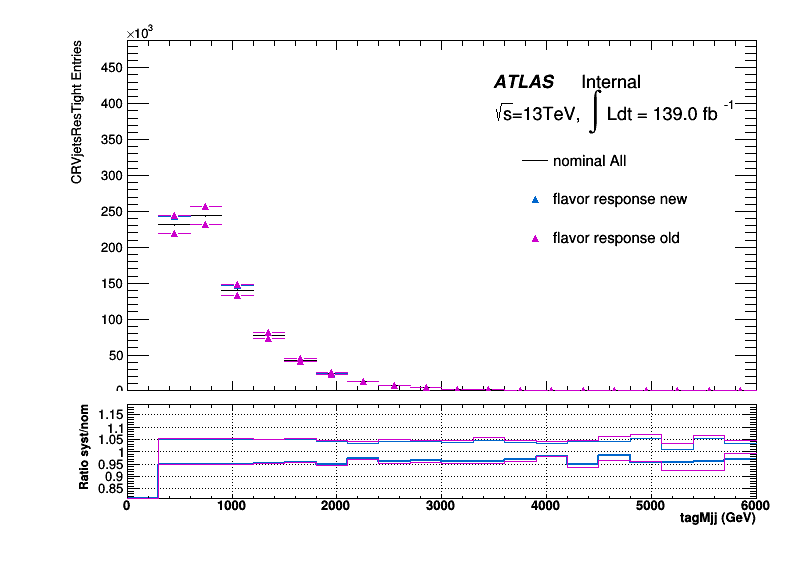
\includegraphics[width=0.4\textwidth]{figures/1lep/FlavorVar/SystFResCRVjetsResTight_All_tagMjj.png}}
%
%        \caption{Comparision between old flavor uncertainties and newly derived flavor uncertainties. Flavor composition uncertainties in particular are greatly reduced.}
%    \label{fig:1LepFlavorVarOldNew}
%\end{figure}



% Gluon fractions as function of pt for 2-lepton channel (nominal)



%%%
\subsection{Tracks uncertainties}
\label{subsec:tracks_uncer}

We incorporate dedicated uncertainties related to track reconstruction, particularly for tracks associated with small-R jets, as outlined in the recommendations on \mbox{\texttt{\href{https://twiki.cern.ch/twiki/bin/viewauth/AtlasProtected/QuarkGluonTagging\#Current_Recommendations}{QuarkGluonTagging}}} and \mbox{\texttt{\href{https://twiki.cern.ch/twiki/bin/view/AtlasProtected/TrackingCPRecsRun2Final\#Track_Systematics_Tools}{TrackingCPRecsRun2Final}}}. 
%Specifically, the ghost-associated track multiplicities of our jets are utilized as inputs to the recurrent layer of the final network.

The procedure in \cite{ATL-PHYS-PUB-2017-009} is used to derive these track multiplicity related uncertainties, of which there are five main components:
\begin{itemize}
    \item fake track efficiency: the uncertainty from the track mis-reconstruction rate;
    \item track efficiency: the uncertainty from the track reconstruction efficiency;
    \item experimental: the uncertainty in charged particle multiplicity, derived as in \cite{CERN-PH-EP-2016-001};
    \item PDF: the theory uncertainty from the parton distribution function;
    \item matrix element: the theory uncertainty from the matrix element calculation;
\end{itemize}
The impacts from these uncertainties are expected to be low.

%%%%%%%%%%%%%%%
%%%We take into account some dedicated uncertainties on the tracks' reconstruction, 
%%%in particular, for the tracks associated to the small-R jets 
%%%\mbox{\texttt{\href{https://twiki.cern.ch/twiki/bin/viewauth/AtlasProtected/QuarkGluonTagging\#Current_Recommendations}{QuarkGluonTagging}}}
%%%\mbox{\texttt{\href{https://twiki.cern.ch/twiki/bin/view/AtlasProtected/TrackingCPRecsRun2Final\#Track_Systematics_Tools}{TrackingCPRecsRun2Final}}}
%%%. 
%%%Indeed, we use the track multiplicities of the ghost associated tracks to our jets as input to the recurrent layer of the final network.
%%%
%%%The procedure in ~\cite{ATL-PHYS-PUB-2017-009}
%%%is used to derive these track multiplicity related uncertainties,
%%%of which there are five main components:
%%%\begin{itemize}
%%%    \item fake track efficiency: uncertainty from track mis-reconstruction rate;
%%%    \item track efficiency: uncertainty from track reconstruction efficiency;
%%%    \item experimental: uncertainty in charged particle multiplicity, derived as in ~\cite{CERN-PH-EP-2016-001};
%%%    \item PDF: theory uncertainty from parton distribution function;
%%%    \item matrix element: theory uncertainty from matrix element calculation;
%%%\end{itemize}
%%%Figures~\ref{fig:1lep_TrackUncCR}, \ref{fig:1lep_TrackUncSR} shows the variations from these sources of
%%%track multiplicity uncertainties for background and signal events in the \olep signal regions.
%%%The impacts from these uncertainties are expected to be low, as they are less than 5\% in the high RNN
%%%bins.

%%%\begin{figure}[ht]
%%%    \centering
%%%        \subfigure[Merged HP SR \ttbar]{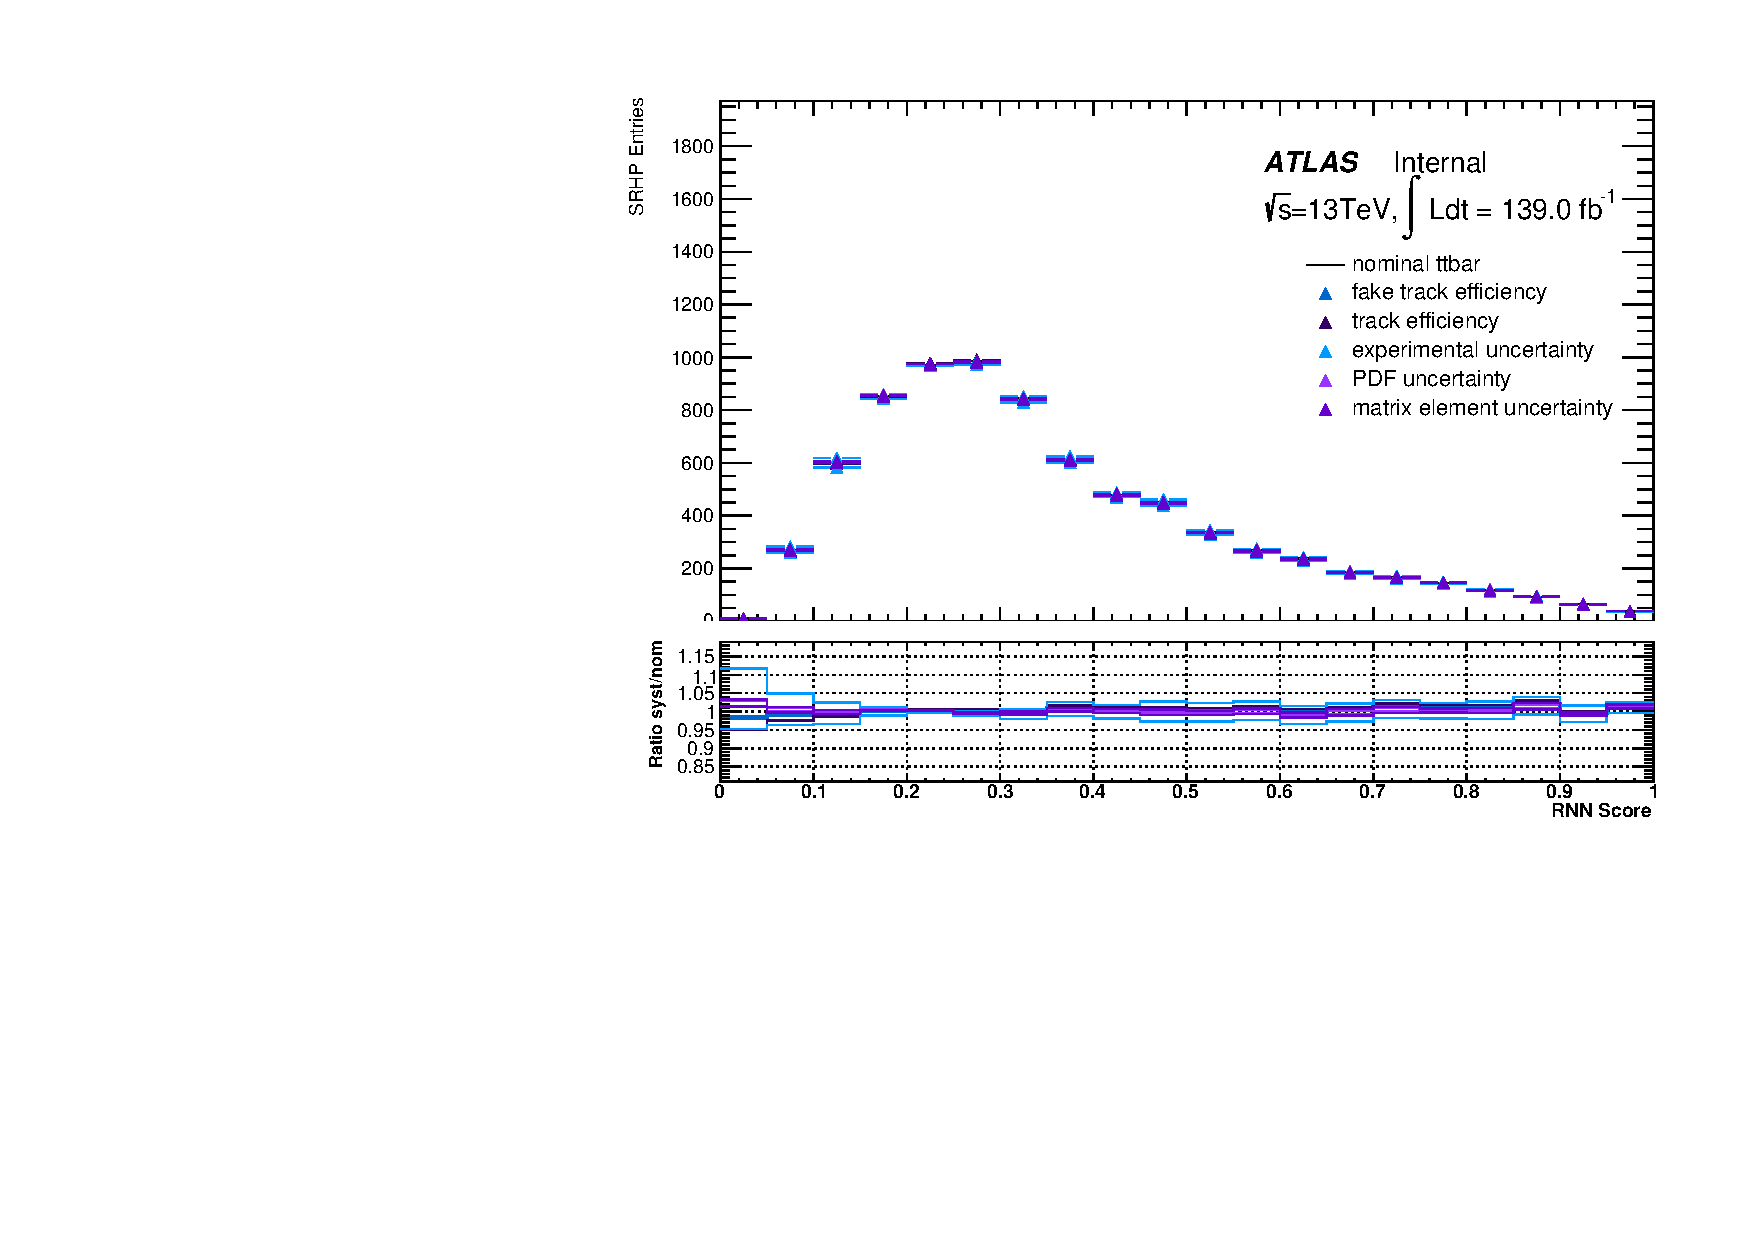
\includegraphics[width=0.45\textwidth]{figures/1lep/TrackSyst/SystQGSRHP_ttbar_RNN.pdf}}
%%%        \subfigure[Merged HP SR W]{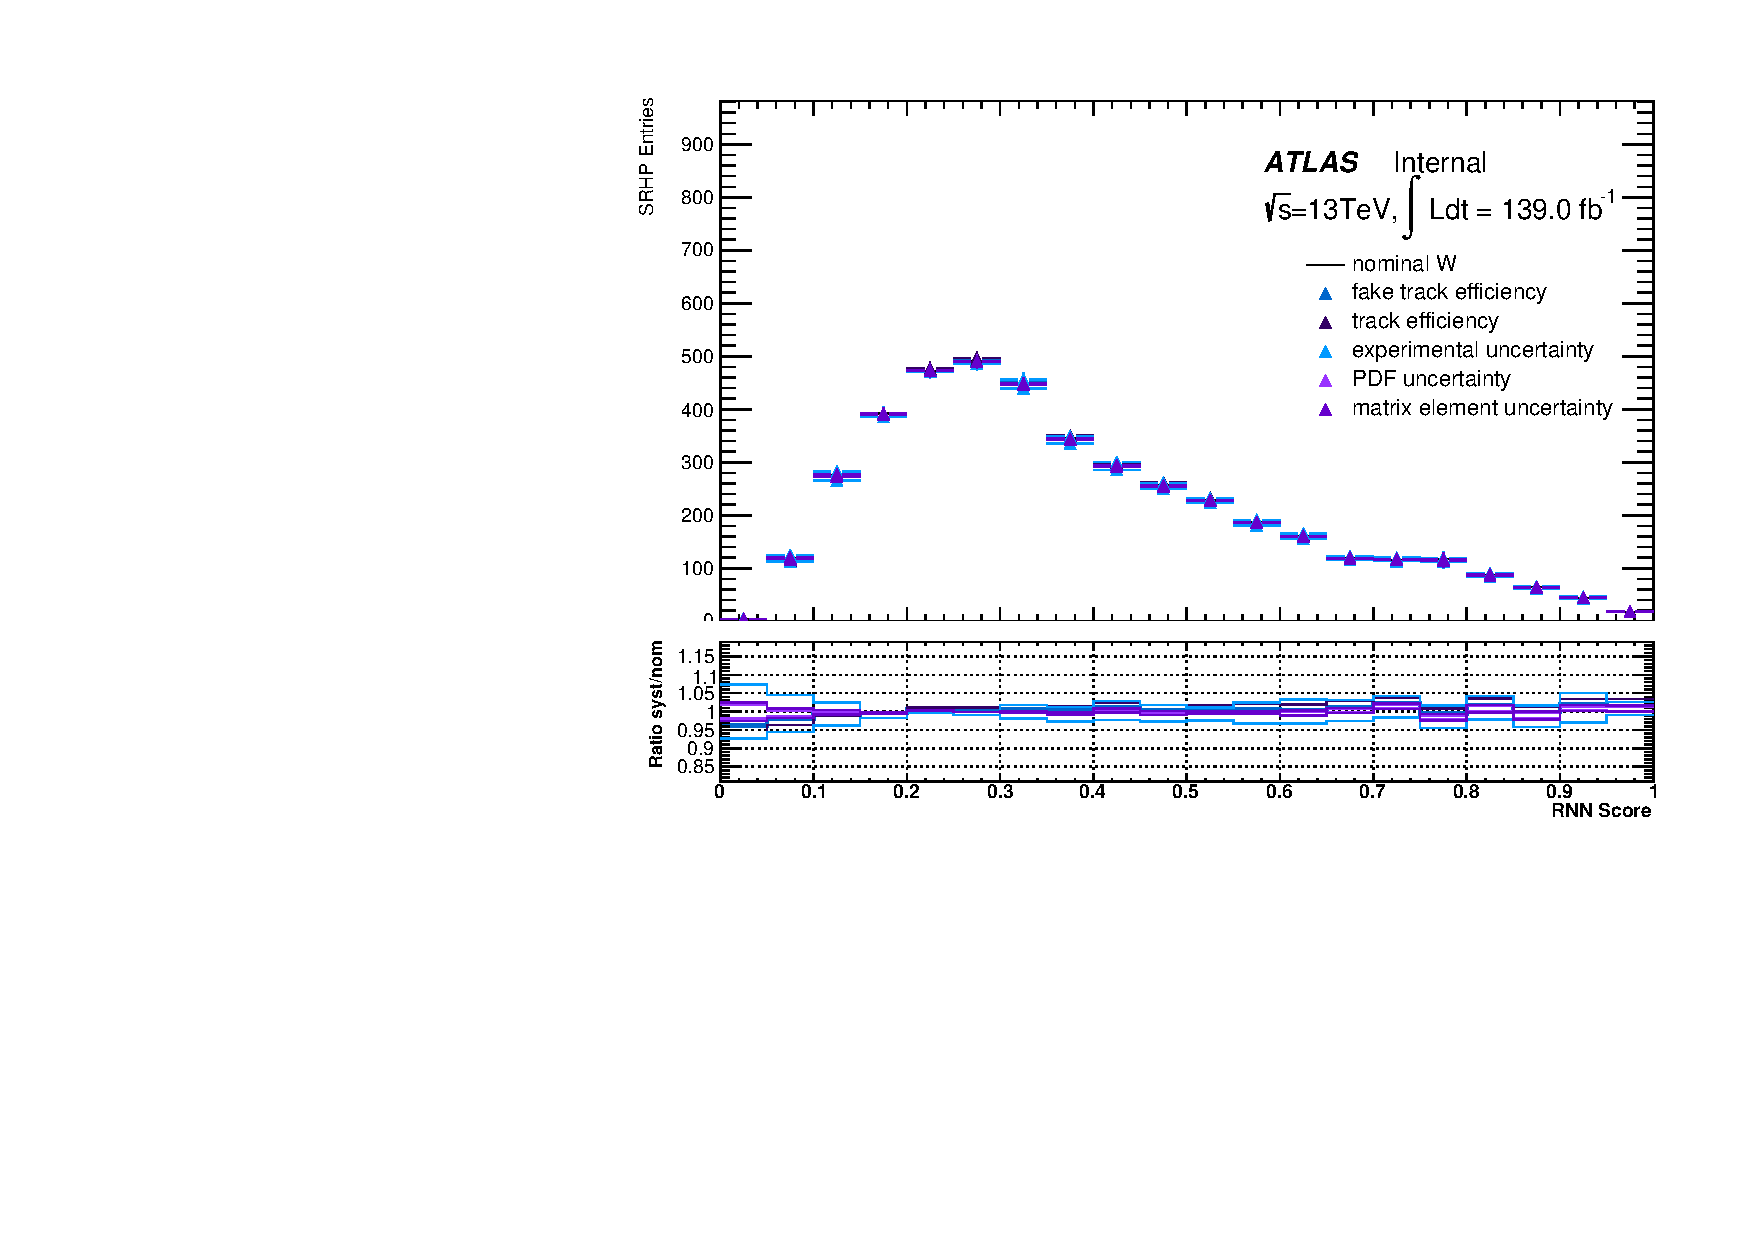
\includegraphics[width=0.45\textwidth]{figures/1lep/TrackSyst/SystQGSRHP_W_RNN.pdf}}
%%%        \subfigure[Merged LP SR \ttbar]{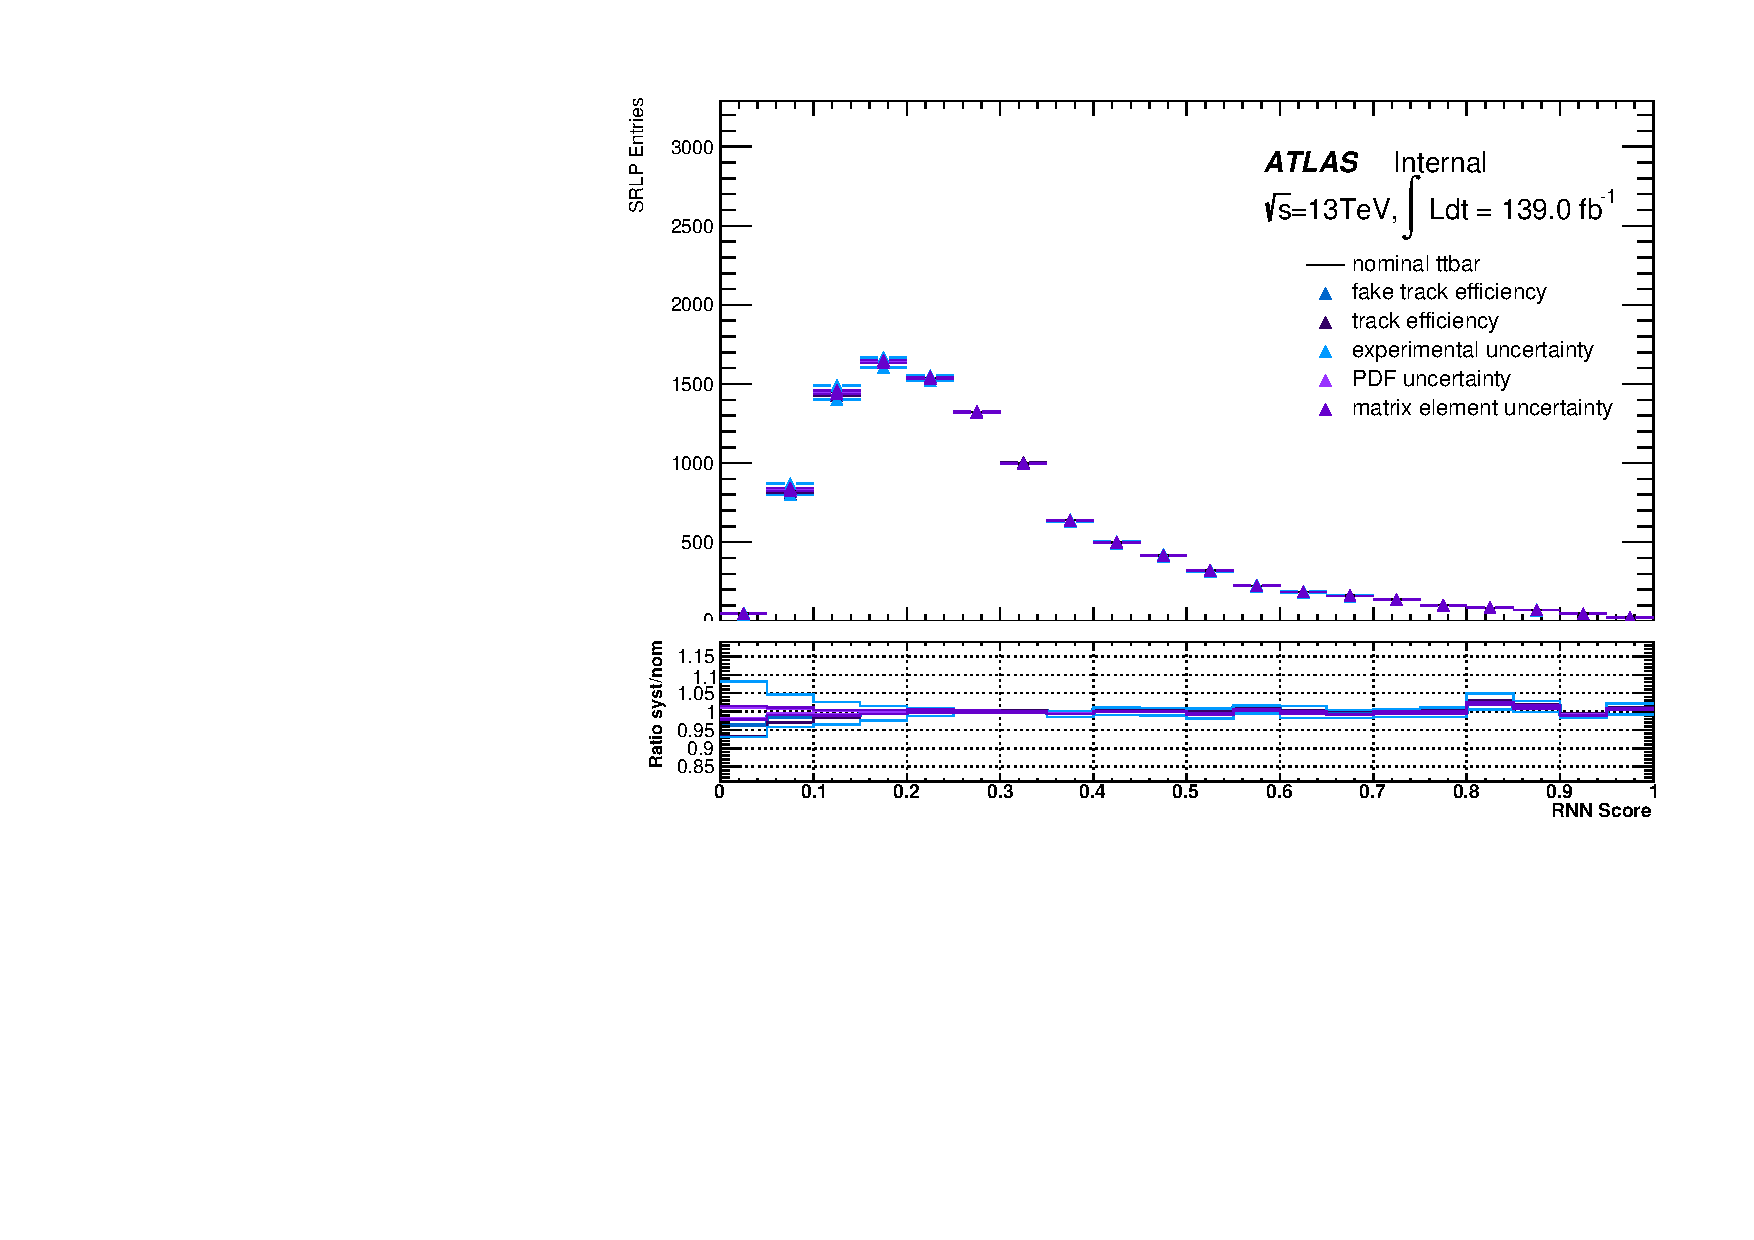
\includegraphics[width=0.45\textwidth]{figures/1lep/TrackSyst/SystQGSRLP_ttbar_RNN.pdf}}
%%%        \subfigure[Merged LP SR W]{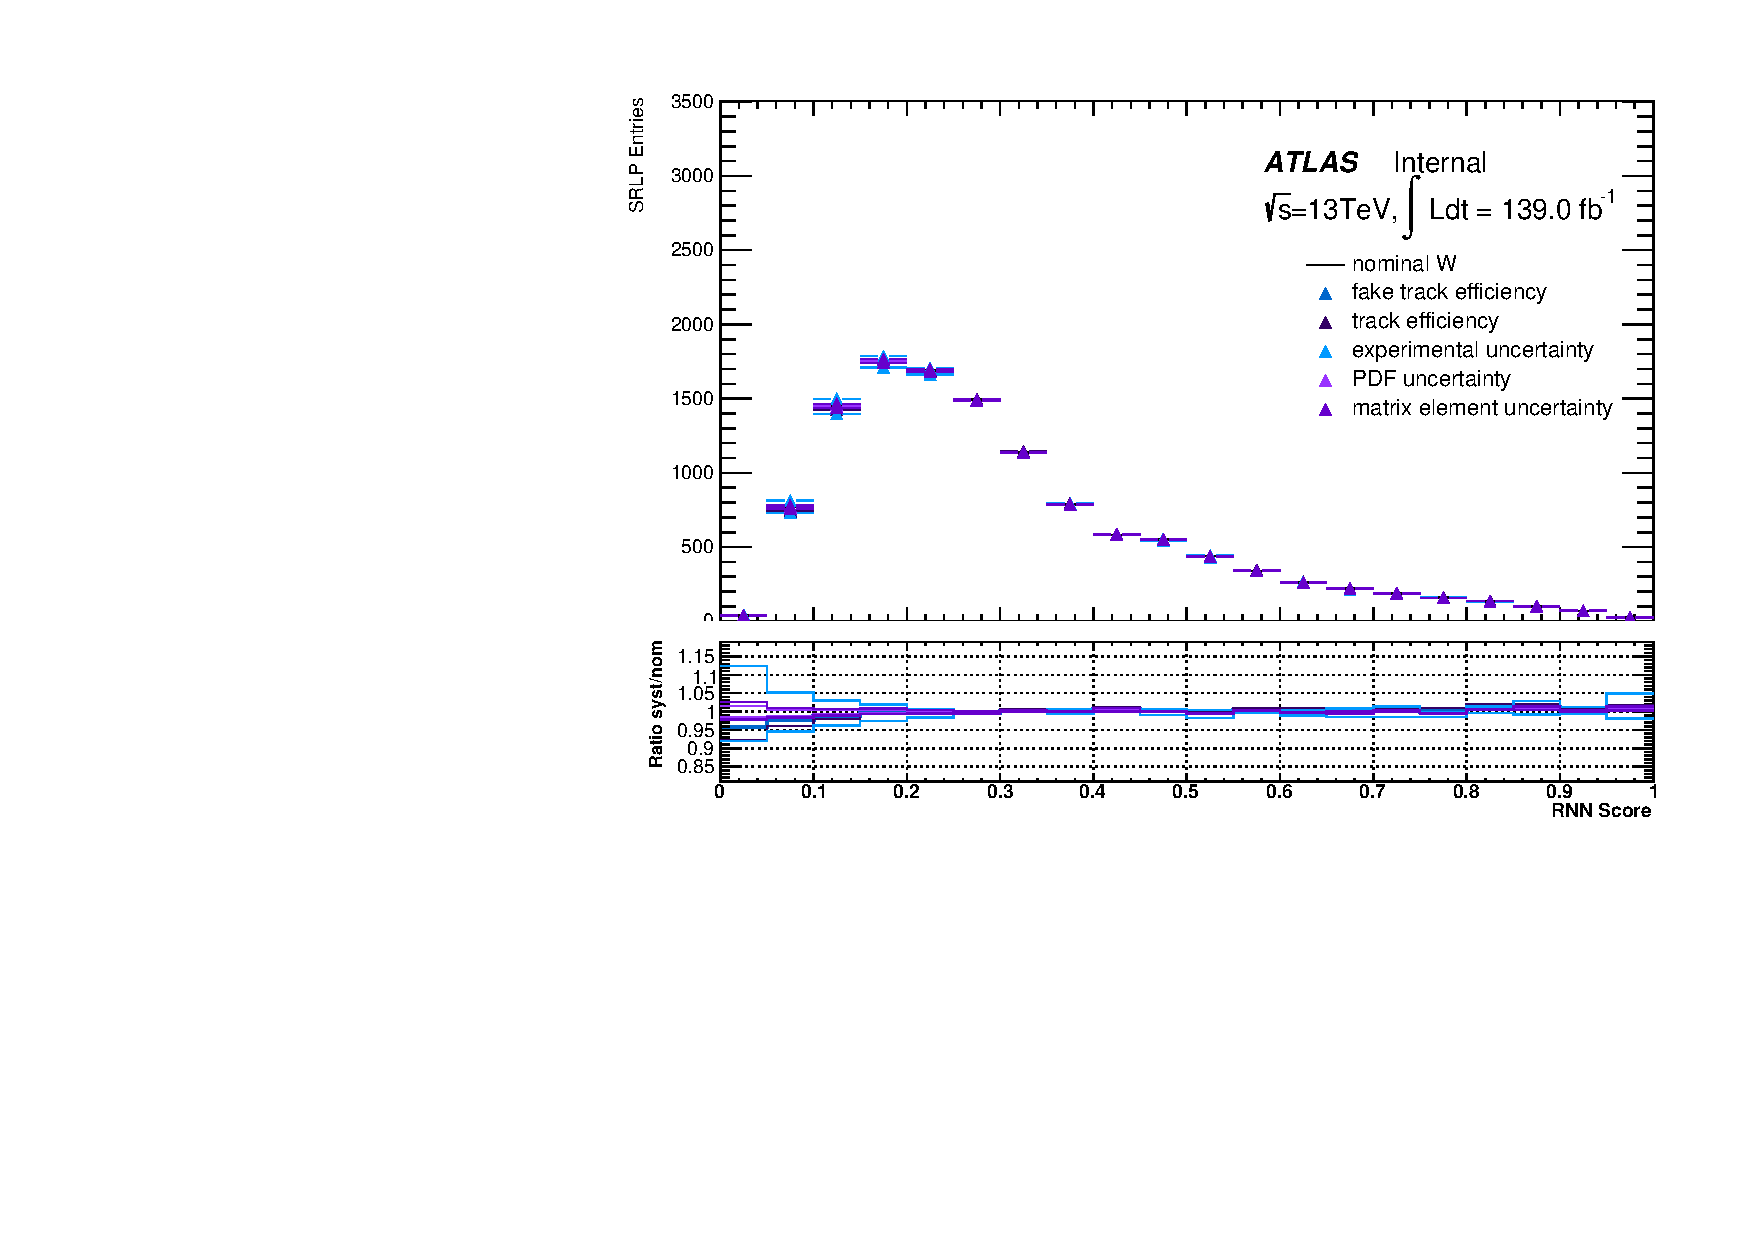
\includegraphics[width=0.45\textwidth]{figures/1lep/TrackSyst/SystQGSRLP_W_RNN.pdf}}
%%%        \subfigure[Resolved SR \ttbar]{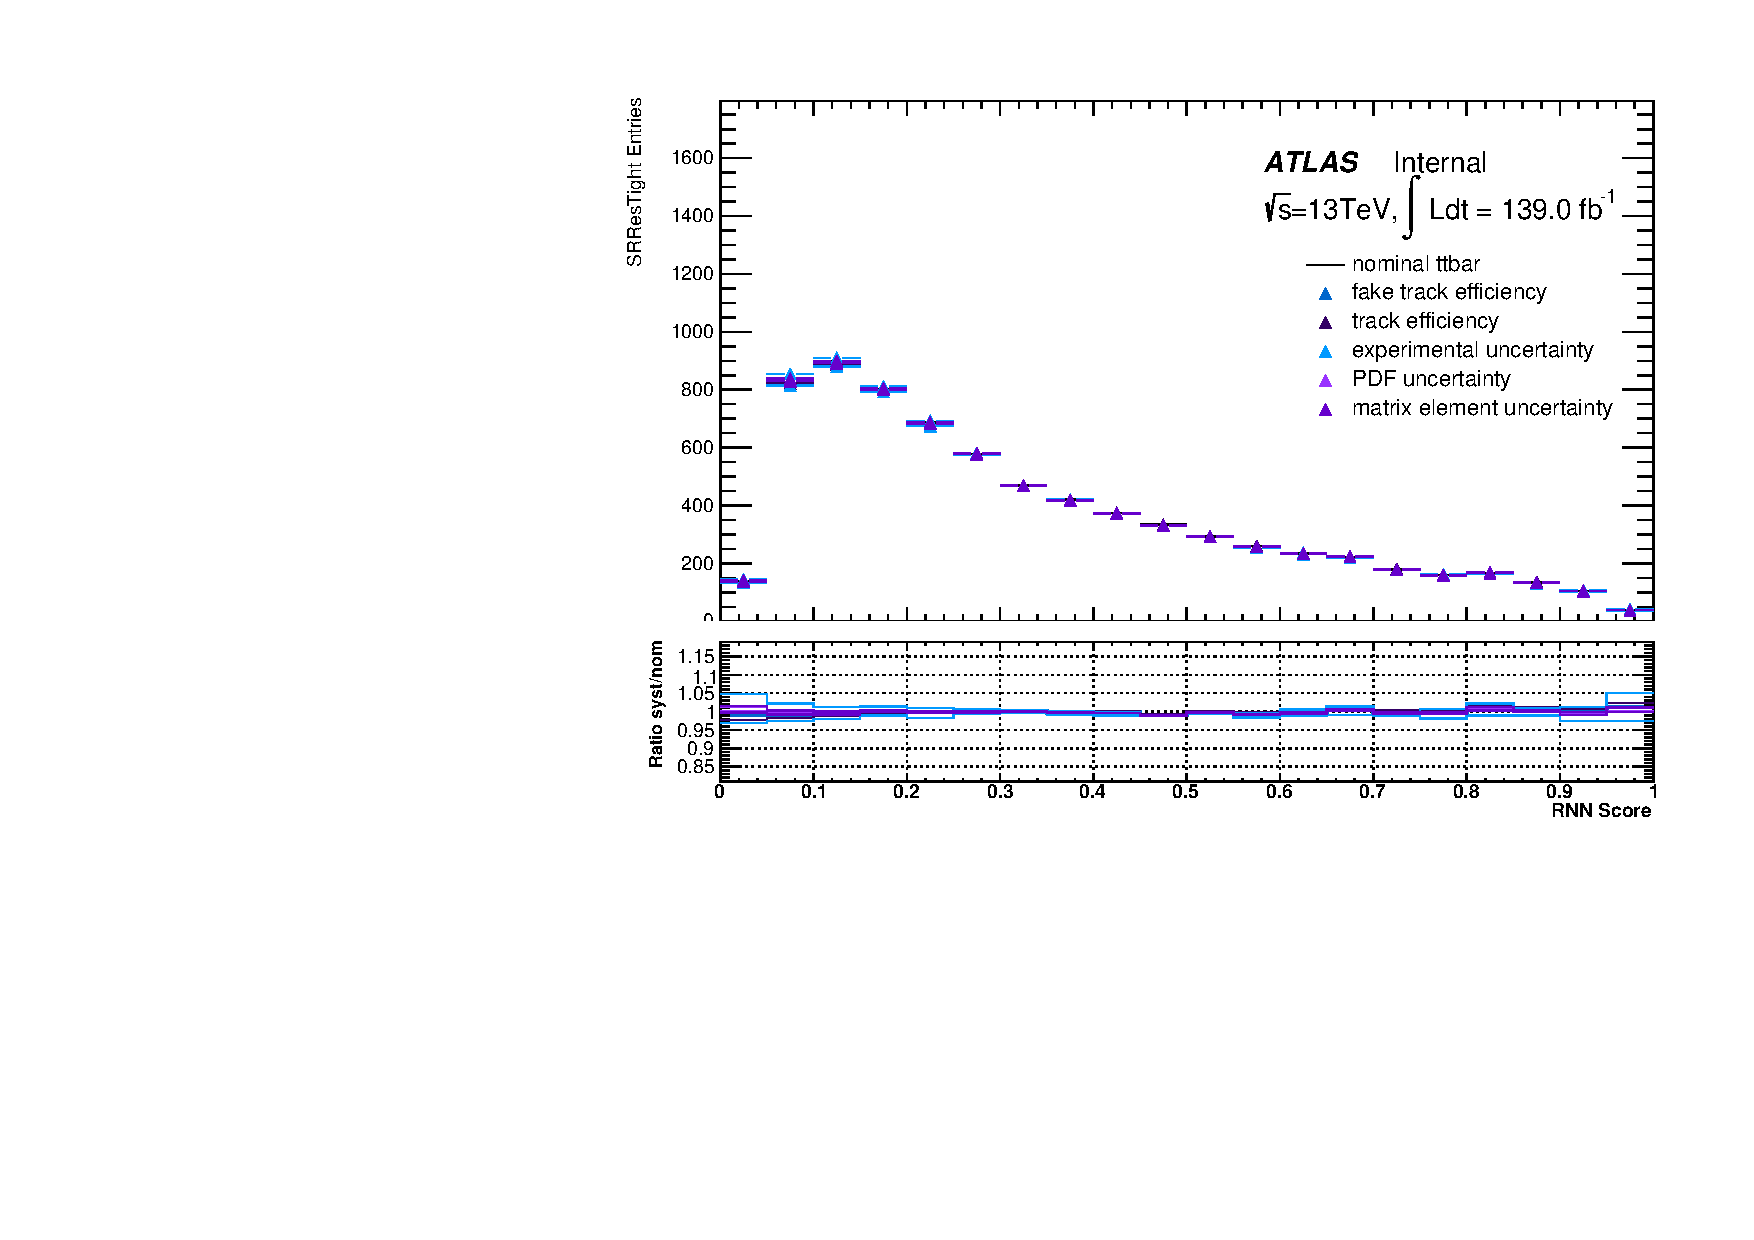
\includegraphics[width=0.45\textwidth]{figures/1lep/TrackSyst/SystQGSRResTight_ttbar_RNN.pdf}}
%%%        \subfigure[Resolved SR W]{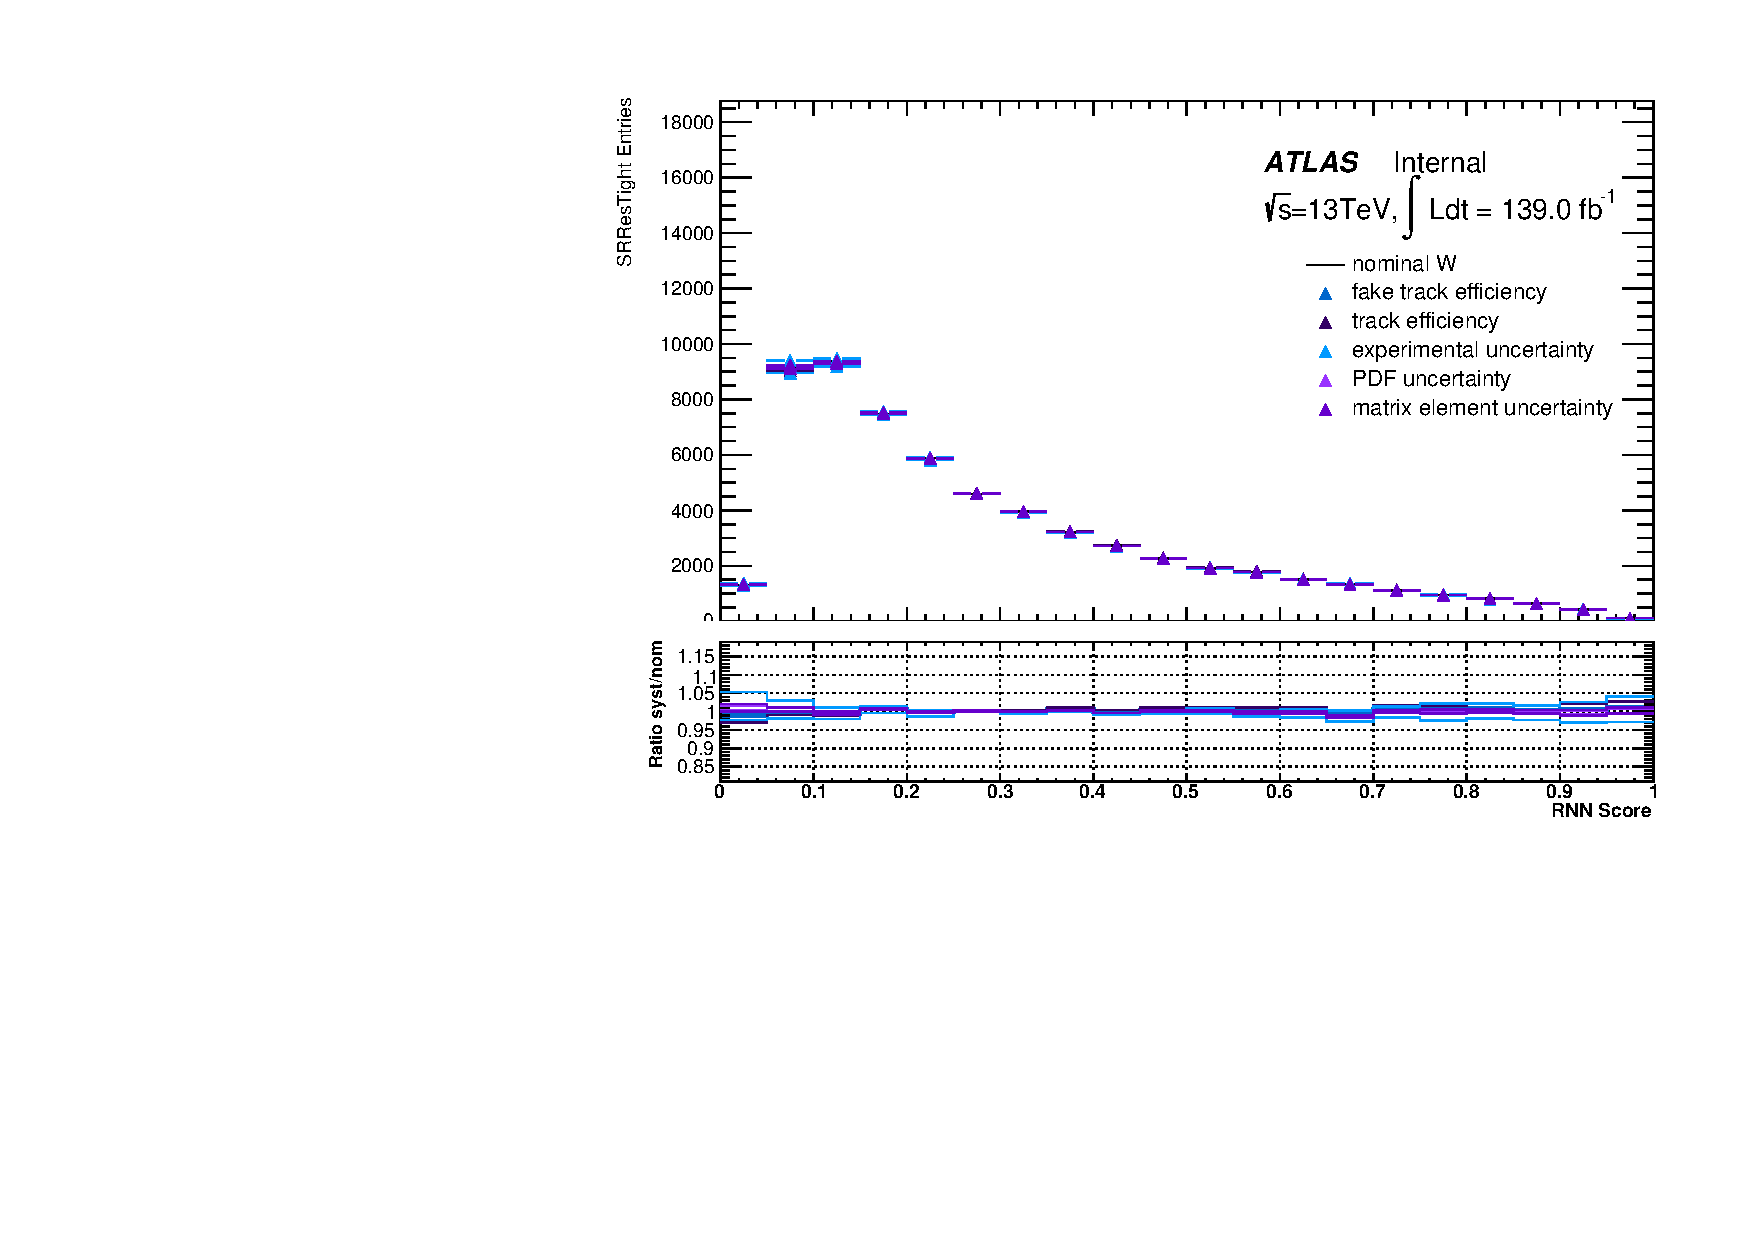
\includegraphics[width=0.45\textwidth]{figures/1lep/TrackSyst/SystQGSRResTight_W_RNN.pdf}}
%%%        \caption{Track multiplicity related uncertainties for \ttbar and \Wjets events in the signal regions. }
%%%    \label{fig:1lep_TrackUncCR}
%%%\end{figure}
%%%
%%%\begin{figure}[ht]
%%%    \centering
%%%        \subfigure[Merged HP SR Signal]{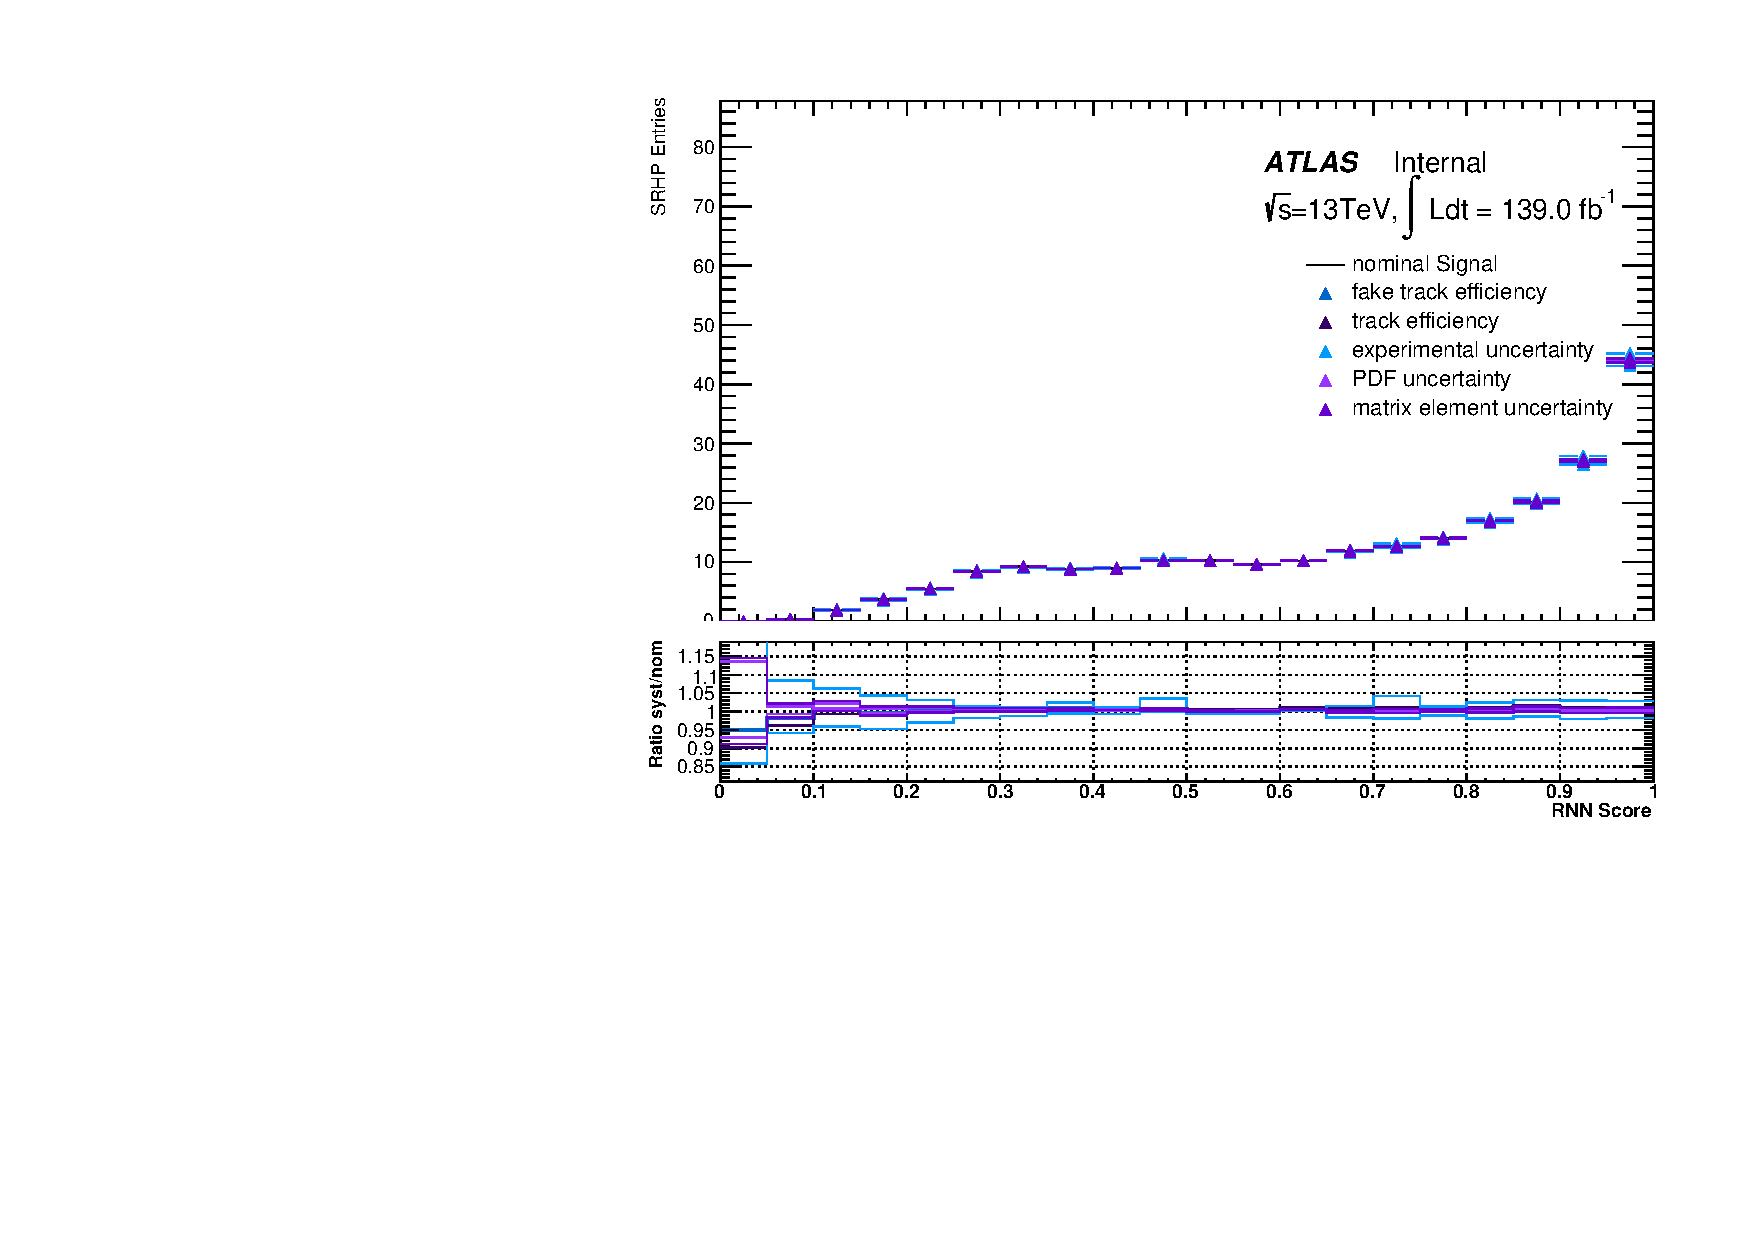
\includegraphics[width=0.45\textwidth]{figures/1lep/TrackSyst/SystQGSRHP_Signal_RNN.pdf}}
%%%        \subfigure[Merged LP SR Signal]{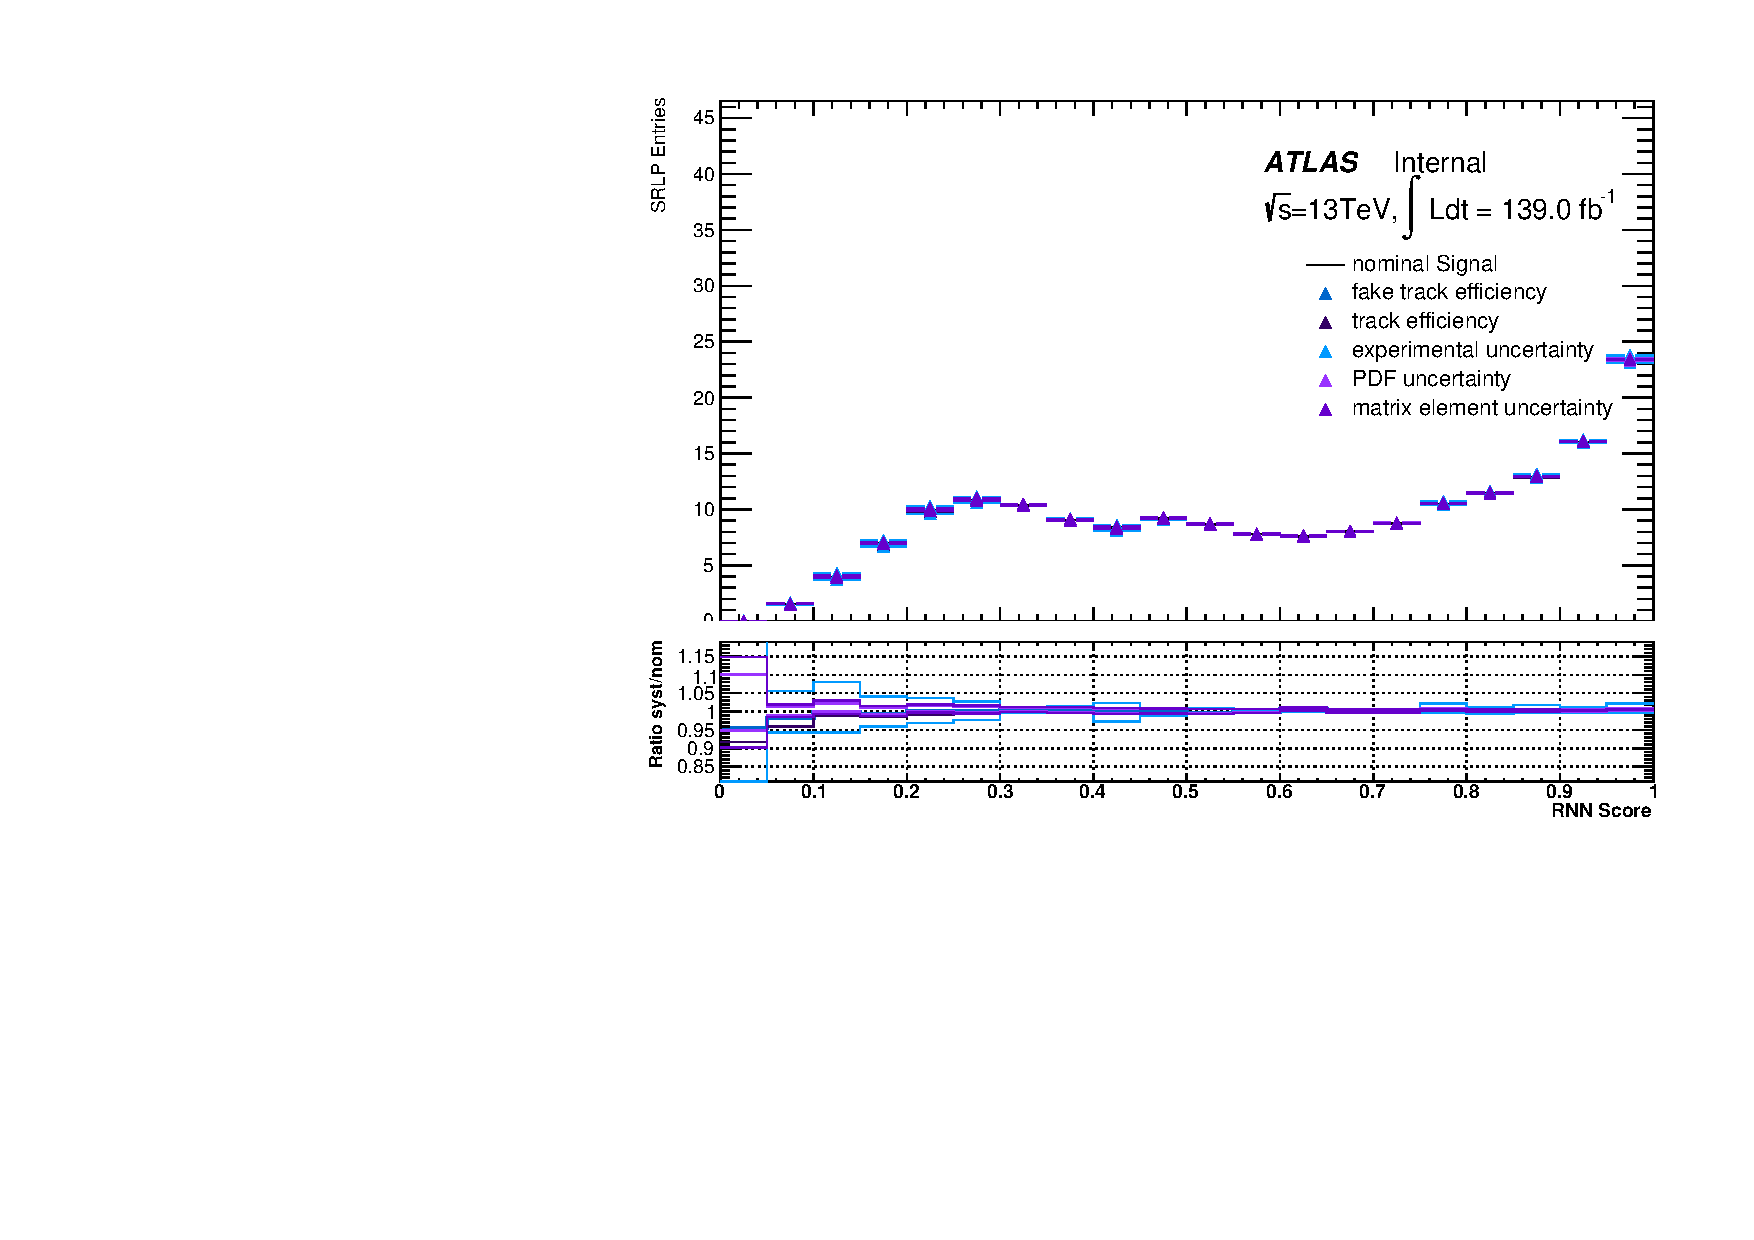
\includegraphics[width=0.45\textwidth]{figures/1lep/TrackSyst/SystQGSRLP_Signal_RNN.pdf}}
%%%        \subfigure[Resolved SR Signal]{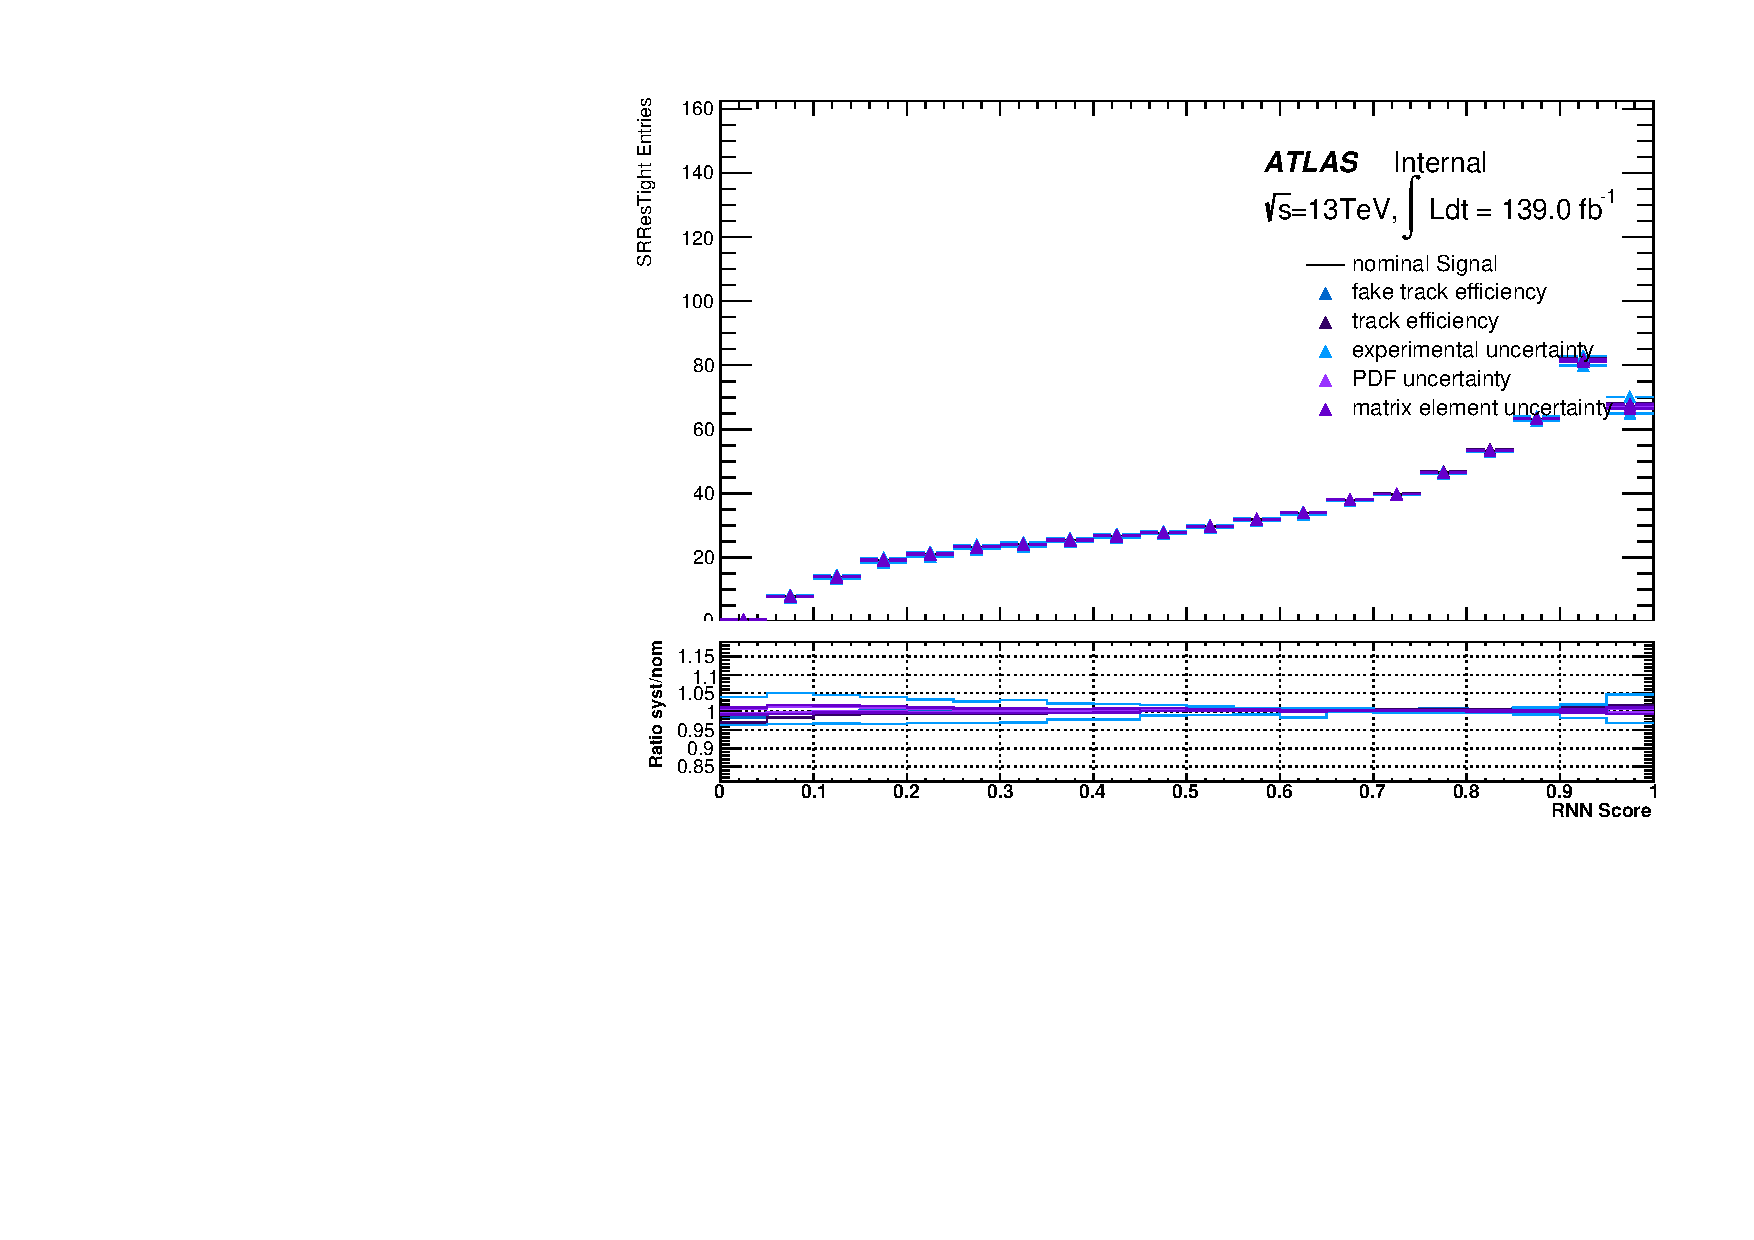
\includegraphics[width=0.45\textwidth]{figures/1lep/TrackSyst/SystQGSRResTight_Signal_RNN.pdf}}
%%%        \caption{Track multiplicity related uncertainties for signal events in the signal regions. }
%%%    \label{fig:1lep_TrackUncSR}
%%%\end{figure}


%both from quick statistics test 
%both from past studies in the VV semi-leptonic resonant search \cite{Bachas:2646593}.


